% https://github.com/dcroote/stanford-thesis-example
% Friday Dec. 3rd noon

% Stanford University PhD thesis style -- modifications to the report style
% This is unofficial so you should always double check against the
% Registrar's office rules
% See http://library.stanford.edu/research/bibliography-management/latex-and-bibtex
% 
% Example of use below
% See the suthesis-2e.sty file for documentation
%
\documentclass[12pt]{report}
\usepackage{suthesis-2e}  % (modified) Stanford thesis style file

% useful packages
\usepackage{graphicx}  % figures
\usepackage{gensymb}  % \degree
\usepackage{siunitx}  % SI units
\usepackage{tabularx}  % nice single page tables
\usepackage{longtable}  % tables spanning multiple pages
\usepackage{hyperref}  % URLs
\usepackage[autostyle, english = american]{csquotes}  % quote orientation
\usepackage{epigraph}
\usepackage[ruled]{algorithm2e}
\usepackage{amsmath}
\usepackage{amssymb}
\renewcommand{\epigraphsize}{\normalsize}
\setlength{\epigraphwidth}{0.9\textwidth}
\MakeOuterQuote{"}

% use png first, otherwise pdf
% (useful for faster compile times, for final submission switch order)
\DeclareGraphicsExtensions{.png,.pdf}

\begin{document}
\title{Machine Learning Based Wavefront Sensing}
\author{David Thomas}
\dept{Computational and Mathematical Engineering}
\principaladviser{Professor Steven Kahn}
\firstreader{Professor Patricia Burchat}
\secondreader{Professor Stephen Boyd}

% no signature or copyright pages in online submission
% (they are added by the library)

% including chapters, no .tex extension necessary
\beforepreface
\afterpreface
\prefacesection{Abstract}
We present a new framework for wavefront sensing for wide-field telescopes. The framework divides the problem into two subproblems that are highly amenable to machine learning and optimization. The first involves making local wavefront estimates with a convolutional neural network. The second involves interpolating the optics wavefront from all the local estimates by minimizing a convex loss function. In this thesis, we develop simulated observations and images from the upcoming Rubin Observatory to refine and assess this framework. Much of this work is also summarized in \cite{2020SPIE11448E..4HT} and \cite{9523024}, although here we describe it in more detail. 

Our unique contributions are as follows. We isolated wavefront sensing problem and decomposed it into two sub-problems. We created benchmark datasets for both sub-problems. We demonstrated a convolutional neural network can predict local wavefront from donut images. We showed that the global wavefront can be interpolated with least squares from the local wavefront estimates. Finally, we developed a wavefront control simulation environment and used it to assess three canonical control strategies.

The algorithm has great practical properties - it is transparent, robust, low latency, and high bandwidth - and achieves stunning performance. In a realistic Rubin mini-survey, the algorithm reduces the total magnitude of the optics wavefront by 66\%, the optics PSF FWHM by 27\%, and increases the Strehl ratio by a factor of 6. The resulting sharper images have the potential to boost the scientific payload for astrophysics and cosmology.
\prefacesection{Acknowledgements}

The idea to pursue graduate school chrystalized when I was working as a quant for Teza Technologies, a small, academic high frequency trading firm. I witnessed first hand how machine learning and low latency technologies were completely up-ending securities trading. Broad shouldered Wall Street suites were being replaced by hackers and math nerds. As machine learning and automation became increasingly powerful tools for our firm, I began to question whether these tools could spur similar advances in physics and cosmology. 

In 2016, I started the Institute for Computational and Mathematical Engineering (ICME) MS program and began working with Philip (Phil) Marshal on high dimensional cosmological inference. In the summer of 2017, Phil introduced me to my eventual advisor, Steven (Steve) Kahn, as someone who could potentially support me for a PhD. I remember our first meeting well. I presented my results. Steve sat there, completely silent. His stern expression gave no indications of his thoughts ... was he even paying attention? After I finished presenting, he asked extremely insightful questions that demonstrated he had been paying careful attention. Indeed, Steve is a great listener. I was also impressed by his creativity and interest in working on problems off the beaten path. Shortly after our first encounter we teamed up to work on star trails, and Steve officially became my PhD advisor. 

Over the past four years we focused primarily on subsecond photometry and wavefront sensing. In both cases, after experimenting with and attempting to extend existing approaches, we were able to develop superior approaches based on machine learning. While these solutions seem very natural in hindsight, it is worth reminding any future PhD students reading this, that we proceeded through many many failed attempts at tackling these problems, received a lot of skepticism around leveraging deep learning initially, before we were finally able to make it work. As Edison says ``I just found 2,000 ways not to make a lightbulb; I only needed to find one way to make it work.'' In this thesis, we focus on our work on wavefront sensing. We point readers interested in our work on star trail photometry to our published and forthcoming papers.

I also would like to thank Patricia Burchat and Aaron Roodman for their guidance and support. As a student from ICME, there were times where I did not feel welcome by the broader physics community. However, Professors Burchat and Roodman always were extremely welcoming and kind. Professor Burchat has been supportive throughout my PhD and provided key feedback to my research efforts and this thesis. Professor Roodman, who developed a previous generation wavefront sensing system, was also an extremely instrumental mentor. My failed attempts to extend his Fourier transform and optimization based method gave me a clearer sense of the key challenges for Rubin and ultimately allowed me to develop a new approach to tackle them. Both of these Professors also asked great questions during my oral defense.

Professor Stephen Boyd was another crucial member of my defense committee. I enjoyed working with Professor Boyd to map the covariance estimation problem for the global wavefront into a convex optimization problem, and on optimal control. This collaboration was a great example of inter-disciplinary research. While Professor Boyd no longer teaches his infamous CME 364A course, Convex Optimization, his recorded 2008 lectures on YouTube have over one million views. These are largely credited as popularizing the subject, and helped to make this my favorite course at Stanford. I believe it provides an unrivalled foundation for machine learning and statistical learning, and encourage any readers to take it - or at least watch Boyd's lectures. 

I would also like to thank my collaborators. Joshua Meyers has been key a mentor and go-to expert on all things optics. His Batoid Python package significantly lowered the hurdles to doing raytracing and really enabled this work. I have also tried to pick up some Joshism's, such as his clean code and notebooks, tendency to use widgets, and clear presentations paced with incredible simulations. 

Federica Bianco has also been a key collaborator on the star trails work. Federica's enthusiasm for science, which ranges from astrophysics to remote sensing to climate change to extraterrestrial technosignatures - is extremely inspiring. She was always willing to meet our projects where they were, and patiently brainstorm and work through the obstacles that come with trying to break new ground. 

I am also extremely grateful to my collaborators at the National Optical Astronomy Observatory in Tucson. Steve helped arange for me to move out there for two quarters in my third year to collaborate with the team and learn the Rubin (then LSST) software stack and wavefront sensing building blocks. The background required for wavefront sensing is not taught in a traditional physics program. In fact, I have still not come across a good \textit{single} reference. Instead one's knowledge must be gleaned from many disparate sources and through experience. Thus, I am very appreciative of the time Bo Xin and Te-Wei Tsai spent with me to impart this wisdom. I also appreciated collaborating with Sandrine Thomas and Chuck Claver on various challenges of the baseline approach the team was developing for Rubin. 

The ICME also played a big role in my development. An ICME graduate can employ more mathematical rigor than most engineers and scientists, and also has strong coding skills. I can't think of better preparation to contribute to innovation in the 21st century. The Directors Margot Gerritsen and Gianluca Laccarino did a great job improving the program throughout my tenure. The former administrative assistant Indira Choudhury was also the spoke that made the institute run, and students graduate. I am forever grateful for her help in this endeavor. 

It has been an incredible priviledge to attend Stanford University. The school has top faculty, a beautiful campus, and ample support and extracurricular activities. It also in the heart of Silicon Valley and can serve as a stepping stone into entrepreneurship. Palo Alto is also a great starting point to explore the broader San Francisco Bay Area. Nowhere else can one surf Pacifica in the morning and meet with venture capitalists on Sand Hill Road in the evening.

I am also very appreciative of Stanford's PhD minor programs. In addition to my PhD in Computational and Mathematical Engineering I was also able to complete a PhD Minor in Physics and PhD Minor in Computer Science. This background has prepared me well to contribute to interfaces between fields where much opportunity remains. I am the first student at Stanford to complete these degrees. 

The past three summers I was able to augment my PhD with three formative experiences. In the summer of 2019, I mentored Stanford undergraduate Emily Li. Emily was a bright and enthusiastic young researcher. She absorbed the optics for wavefront sensing like a sponge. This experience taught me how to clearly communicate expectations, share the joy of science, and teach foundational skills. The experience encouraged her to pursue a career in physics. Nothing is more rewarding than seeing one's mentees succeed.  

In summer 2020, I interned as a Quantitative Researcher in the Global Quantitative Strategies business at Citadel Investment Group. It was great to see how state of the art quantitative hedge funds operate and compare and contrast the methods used here with those used during my time in high frequency trading. While I cannot go into detail about my work there due to a strict non-disclosure agreement, I can say that there is a lot of value in being fluent in the mathematics behind statistical learning models as well as being a strong programmer and knowing how to accelerate and improve these models and their training on modern compute infrastructure. Again, the ICME combination of mathematical rigor and computational engineering was superb preparation. This experience was also a great reminder of how challenging it is to beat the market. Even with a team of hundreds of highly accomplished PhD researchers, state of the art software and resources, and the accumulation of millions of signals and research findings ... it is difficult to break even. I suspect people who have not experienced this world first hand, and the repeated failures that accompany this amibitious goal, with billions of dollars on the line, cannot truly appreciate how efficient markets really are. Retail trading and investing is pure speculation - and a losing game. 

In summer 2021, I interned as a Machine Learning Engineer on the Instagram Ads Ranking and Delivery team at Facebook. I really enjoyed researching and developing large scale recommender systems. These systems, used in everything from Google's search engine to prioritizing content on Facebook's home feed, are some of the most critical components of large tech businesses and the modern internet. The computational resources and datasets available at companies like Facebook are so superior to those in academia that to perform cutting edge work in this field almost necesitates one to work for a large tech company. Some of my colleagues were former faculty members who moved from academia to research roles at Facebook in order to get around this discrepancy and continue producing impactful research. It seems like it will be increasingly difficult for academia to retain top talent in these fields: large scale recommender systems and machine learning more broadly.  

My family has always been incredibly supportive. My father David \textit{Evan} Thomas served in the United States Navy for 25 years. I am incredibly proud of his committment and dedication to his country. When I was growing up, we would stay with relatives over the holidays so he could work over his vacations to earn enough money to send my sister to a private high school. That was a good investment, because today my sister Danielle Thomas has become a very successful orthopedic surgeon. She is a tough cookie - her favorite tool is the bone saw - and has no problem exceling in a field that is over 90 percent male. She also is a voracious reader. She read over one hundred books in each of the last two years. My mother Valerie Thomas was my original teacher during infancy and has encouraged my pursuits ever since. During my PhD, she would regularly visit the bay area and would send me care packages. She has become an incredible painter. Her paintings decorate my walls; guests tend to be surprised that the artist is, in fact, my mother.

Finally, I would like to give the utmost thanks to my wife Madeleine Scott. We met as undergraduates at MIT and started dating in 2012. She briefly worked at a biotech startup before pursing both an MD and a PhD at Stanford through the eight year, fully funded, and \textit{extremely} competitive Medical Scientist Training Program. She is an incredibly kind person that feels so much for other people that she cannot watch dramatic movies. She loves helping others solve problems and will be an incredible physician. She is also the most talented young scientist that I know. This past year she has had two papers accepted to the revered journal Nature. I am very fortunate to be her collaborator in life. 

My wife's parents Frances Donovan and Gary Scott have been incredibly supportive throughout our relationship and especially during the Covid-19 pandemic. During Covid we have stayed with them in Berkeley for months at a time. Their active lives, copious reading, fascinating conversations, and respect for each other set a great example. While, Gary, a Physics PhD who now works as a molecular biology researcher, enjoys shooting down dark matter, lambda-CDM, and other tennets of modern cosmology - I cannot thank him and Frances enough for letting me marry their daughter. 

Recently, we welcomed a new member into our family. Kyver Blaze Thomas was born at 3:48 pm on July 24th at the Lucile Packard Children's Hospital. We are absolutely smitten new parents. Kyver is already good-natured like his mom, and inquisitive like his dad. Perhaps one day he will read this thesis.

% \include{ch_intro}
\part{Machine Learning Based Wavefront Sensing}
% Full title as you would like it to appear on the page
\chapter{A New Paradigm For Wide-Field Wavefront Sensing}
\label{chap:new_paradigm}
% Short title that appears in the header of pages within the chapter
\chaptermark{A New Paradigm}

\epigraph{What is the most important theme in computer science? [Class responds.] No. It is \textit{abstraction}.}{John Ousterhout in CS 140: Operating Systems, 2020}

\section{Challenges with Previous Approaches}

Keeping telescopes in focus is an art as old as the instruments themselves. Their widespread use spurred the development of theories of optics and aberrations. In 1678, the famed Dutch physicist Christian Huygens proposed that every point that interacts with light may be regarded as the source of a new spherical wave. In 1818, the French physicist Augustin-Jean Fresnel incorporated interference into this model. The resulting Huygens-Fresnel principle is still a widely taught model for wave propagation and provides the physical intution behind reflection, refraction, and diffraction. The paradigm also introduced the notion of the wavefront.

A wavefront is a two dimensional surface over which the phase of the wave is constant. We also overload this diction to refer to aberrations, or two dimensional spatial offsets from a reference wavefront. Figure \ref{fig:wavefront} shows example aberrations to planar and spherical reference wavefronts. 

\begin{figure}[hbt!]
\centering
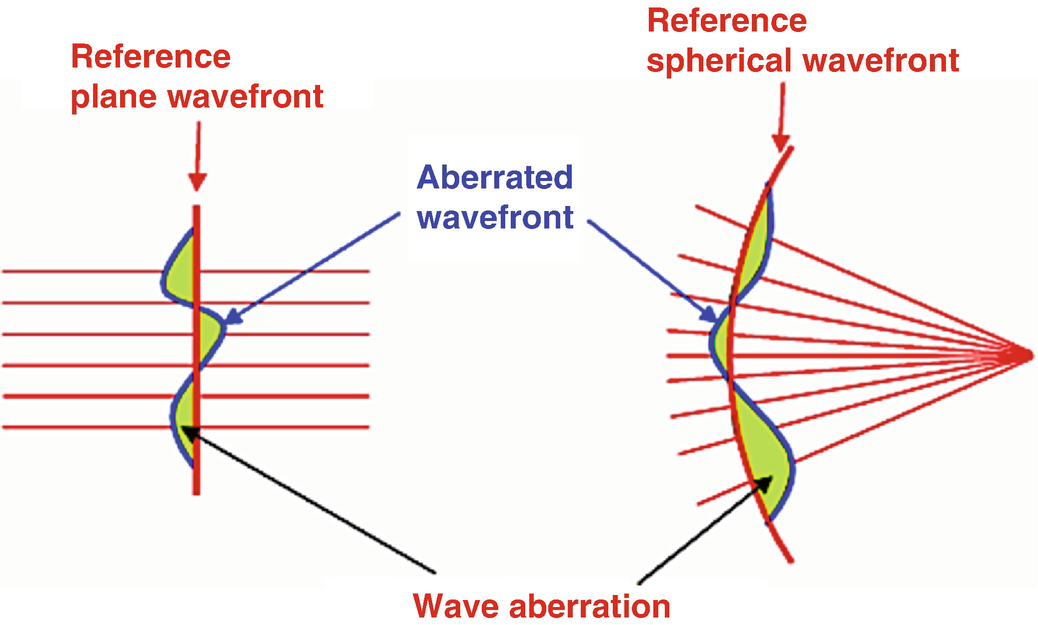
\includegraphics[width=14cm, keepaspectratio]{figs/new_paradigm/wavefront.png}
\caption[Wavefront and Wavefront Aberrations]{Example aberated planar and spherical wavefronts. The horizontal red lines show the direction of propagation. The vertical red line shows the reference wavefront and the blue line shows an example aberrated wavefront. Source: \cite{wavefront_fig}. }
\label{fig:wavefront}
\end{figure}

Wavefronts are useful because the wavefront aberrations in different planes, and through time, largely characterize the image quality of an optic. In the case of ground based telescopes, there are three primary contributions to image quality: the atmosphere, the telescope, and the camera. The field of \textit{adaptive optics} is concerned with controlling deformable mirrors to the optical path to correct for aberrations induced by atmospheric turbulence on 10-100Hz frequencies. However, for wide field telescopes with fields of view on the order of a degree, a common corrections is not possible for the entire field of view. In this context we are primarily concerned with \textit{active optics} which strives to correct the aberrations due to the telescope. New methods of wavefront sensing for active optics is the focus of the first part of this thesis.

One way to characterize the optics of a telescope is through path length differences. For every position in the image plane, we can measure the path differences to points in the entrance pupil. An alternative way to mathematically express this is through an aberrated wavefront defined at the entrance pupil for each position in the image plane. Then the imaging properties can be computed with Fourier Optics. We refer readers who would like to understand this relation further to Goodman's classic Fourier Optics text \cite{goodman2005introduction}. 

There are two thematic approaches to wide field wavefront sensing: zonal and modal. In the zonal approach, the entrance pupil is partitioned into an array of subaperatures. In each of these zones, the wavefront is characterized by its optical path length, local gradient, or local curvature. The wavefront measurement improves with more partitions. The Shack-Hartmann sensor and shearing interferometer are the two most common zonal approaches.

The modal approach treats the wavefront aberration, at a given point in the image plane, as a sum of low order polynomials defined over the entrance pupil. This wavefront measurement improves with higher order polynomial measurements. Modal approaches typically rely on strategically defocused wavefront sensors. The Rubin Observatory focal plane was designed with a modal approach in mind as it does not require lenselets or tweaks to the beam. As described in chapter \ref{chap:aos}, the Rubin focal plane contains four corner wavefront sensors specifically for this purpose.

There are two previously described approaches to wavefront sensing that are relevant for Rubin. The first, by Roodman et. al. \cite{2014roodman}, is the algorithm used for the Dark Energy Camera on the Blanco Telescope \cite{darkenergycamera}. It is based on the Fraunhofer diffraction integral:

\begin{equation}\label{eqn:fraunhofer}
I(x,y) \propto |\mathcal{F}\{P(\rho, \theta \exp(2\pi i W(\rho, \theta) / \lambda))\}|^2
\end{equation}

\noindent where $I$ is intensity; $\mathcal{F}$ is the two-dimensional Fourier transform; $P$ is the pupil function; $W$ is the wavefront; $\lambda$ is the wavelength; and $x,y$ and $\rho, \theta$ parameterize the image and pupil planes respectively. The wavefront is modeled as a sum of orthonormal Zernike polynomials:

\begin{equation}\label{eqn:zernike_decomp}
W(\rho, \theta) = \sum_i a_i Z_i(\rho, \theta)
\end{equation}

\noindent Starting from a set of telescope control parameters, the wavefront coefficients can be computed. Then the Fraunhofer diffraction integral can be used to generate a corresponding intensity image. The difference between the donut images and the images from the forward model,

\begin{equation}\label{eqn:loss}
\mathcal{L} = \sum_{\text{donut d}}||I_{\text{d,true}} - I_{\text{d,forward}}||_2^2
\end{equation}

\noindent can be used as a loss function. Then we can estimate the telescope parameters by using an optimizer to find the parameters that minimize this loss function. This works well when there are a few non-degenerate parameters and the problem remains approximately convex.

While this approach has been successfully applied to the Blanco Telescope, there are two impediments to applying it to the Rubin Observatory. The first is that Rubin has much higher dimensionality and complete degeneracy between some of the parameters of interest. The Blanco Telescope is a prime focus telescope with a single mirror; the Rubin Observatory is a modified Paul-Baker telescope with three mirrors. The Blanco active optics sytem controls 8 parameters; the Rubin active optics system strives to control 50 parameters. The Rubin control parameter optimization surface is highly nonconvex. In addition to these theoretical hurdles, the fast beam of the Rubin optics also necesitates much larger fourier transforms pushing the runtime of the algorithm beyond the 15 seconds we are targeting (see next chapter for more details). 

The second approach is based on the transport of intensity equation (TIE):

\begin{equation}\label{eqn:tie}
\frac{\partial I}{\partial z} = -(\nabla I \cdot \nabla W + I \nabla^2 W)
\end{equation}

\noindent where $z$ is the optical axis. It builds on the curvature wavefront sensing technique developed by Francois, Claude, and Nicolas Roddier \cite{curvaturesensing}. Their key insight was that $\frac{\partial I}{\partial z}$ can be approximated by subtracting two donut images on different sides of focus. Then $W$ in the TIE equation can be solved for in Fourier space or with a Zernike polynomial series expansion. The large central obscuration, fast $f$-number, off-axis distortion and vignetting, and different field positions of intra and extra-focal donuts are four challenges to using curvature sensing for Rubin. Xin et. al. \cite{2015Xin} proposed solutions and extended curvature sensing to estimate the Rubin optics wavefront at four field positions. Below we give a high-level summary of the operations this algorithm performs, on a single wavefront sensor, to estimate the wavefront at the center of the corresponding wavefront sensor:

\begin{enumerate}
\item Crop $N$ pairs of intra-focal and extra-focal donuts \\$\{(D_{\text{intra},1},\ D_{\text{extra},1}), \dots, (D_{\text{intra},N},\ D_{\text{extra},N})\}$.
\item Make initial wavefront estimates $W_0 = 0,\ W_1 = \text{guess}$.
\item Set $i = 1$.
\item While $||W_i - W_{i-1}||_2^2 < \text{tolerance}$ repeat,
\begin{enumerate}
\item Apply nonlinear transformation $f$ which migrates donut image from its field position to the center of the wavefront sensor, based on current wavefront estimate $W_i$. We have $\{(D_{\text{intra},1}^\prime,\ D_{\text{extra},1}^\prime), \dots, (D_{\text{intra},N}^\prime,\ D_{\text{extra},N}^\prime)\}$ where $D_{*,k}^\prime = f(D_{*,k}, W_i)$.
\item Apply correct $g$ for intensity and vignetting differences between the pairs of donuts. We have $\{(D_{\text{intra},1}^{\prime\prime},\ D_{\text{extra},1}^{\prime\prime}), \dots, (D_{\text{intra},N}^{\prime\prime},\ D_{\text{extra},N}^{\prime\prime})\}$ where $D_{*,k}^{\prime\prime} = g(D_{*,k}^\prime, W_i)$.
\item Set $(\partial_z I)_k \propto D_{\text{intra},k}^{\prime\prime} - D_{\text{extra},k}^{\prime\prime}$.
\item Solve TIE for $W_{i+1}$ with $(\partial_z I)_k$ by series expansion.
\item Set $i = i + 1$.
\end{enumerate}
\item Return $W_i$ as wavefront for the center of the wavefront sensor.
\end{enumerate}

\noindent Afer this process the algorithm uses the wavefront estimates at the center of the four corner wavefront sensors to constrain 50 telescope control parameters (these parameters are described in the next chapter). 

This approach has been developed by a dedicated team over the last decade. Parts of the algorithm, such as step 4 (d) are mature and have been validated on real data \cite{cwfs_comparison}. However, despite significant effort, the code for the full algorithm on Rubin remains incomplete. Thus it is difficult to benchmark or compare to alternatives.

The primary challenge on theoretical grounds is the convergence. There are no convergence gaurentees. The wavefront estimate may not improve between the iterations in step 4. Some tests suggest that the algorithm typically converges for small perturbations to the nominal optics configuration. However, for large perturbation the transformations $f$ and $g$ will have more error. A different strategy might be required.

The algorithm is also fairly computationally expensive. It takes approximately 15 seconds to perform 10 iterations of step 4 on 10 pairs of donuts. However, a typical wavefront sensor image contains close to a thousand donut images. A lot of potentially useful donut information is ignored.

There are also a few challenges on practical grounds. The functions $f$ and $g$ used in step 4 depend on the wavefront estimate and are fairly complicated. This makes the algorithm challenging to interpret and debug. Also, since $f$ and $g$ depend on the wavefront estimate, it is difficult to characterize the error in the full algorithm, because each step depends on the preceeding steps. 

After spending a year supporting efforts to implement this algorithm, I realized the prudence in developing an alternative approach. I sought to develop an algorithm that was simple, transparent, robust, low-latency, and high-throughput. The next two sections develop two key paradigms behind the algorithm.

\section{The Double Zernike Polynomials}

The Zernike polynomials are a sequence of polynomials $\{Z_i\}$ that are widely used to characterize wavefronts in optics \cite{zernike}. They are defined over a unit disk, or annulus, and normalized such that

\begin{equation}\label{eqn:zernike_norm}
\int_{R_{\text{inner}}}^{R_{\text{outer}}} \int_0^{2\pi} Z_i(\rho,\theta)Z_j(\rho,\theta)d\rho d\theta = \delta_{ij}
\end{equation}

\noindent Figure \ref{fig:zernike} shows the first 21 Zernike polynomials. For characterizing a wavefront in the pupil plane we follow the convention of using $Z_4-Z_{21}$ by Xin et. al. \cite{2015Xin}. The first three polynomials are ignored because while they effect the position of the image, they do not impact the image quality. The polynomials beyond 21 are ignored because they are only weakly excited by typical Rubin perturbations.

\begin{figure}[hbt!]
\centering
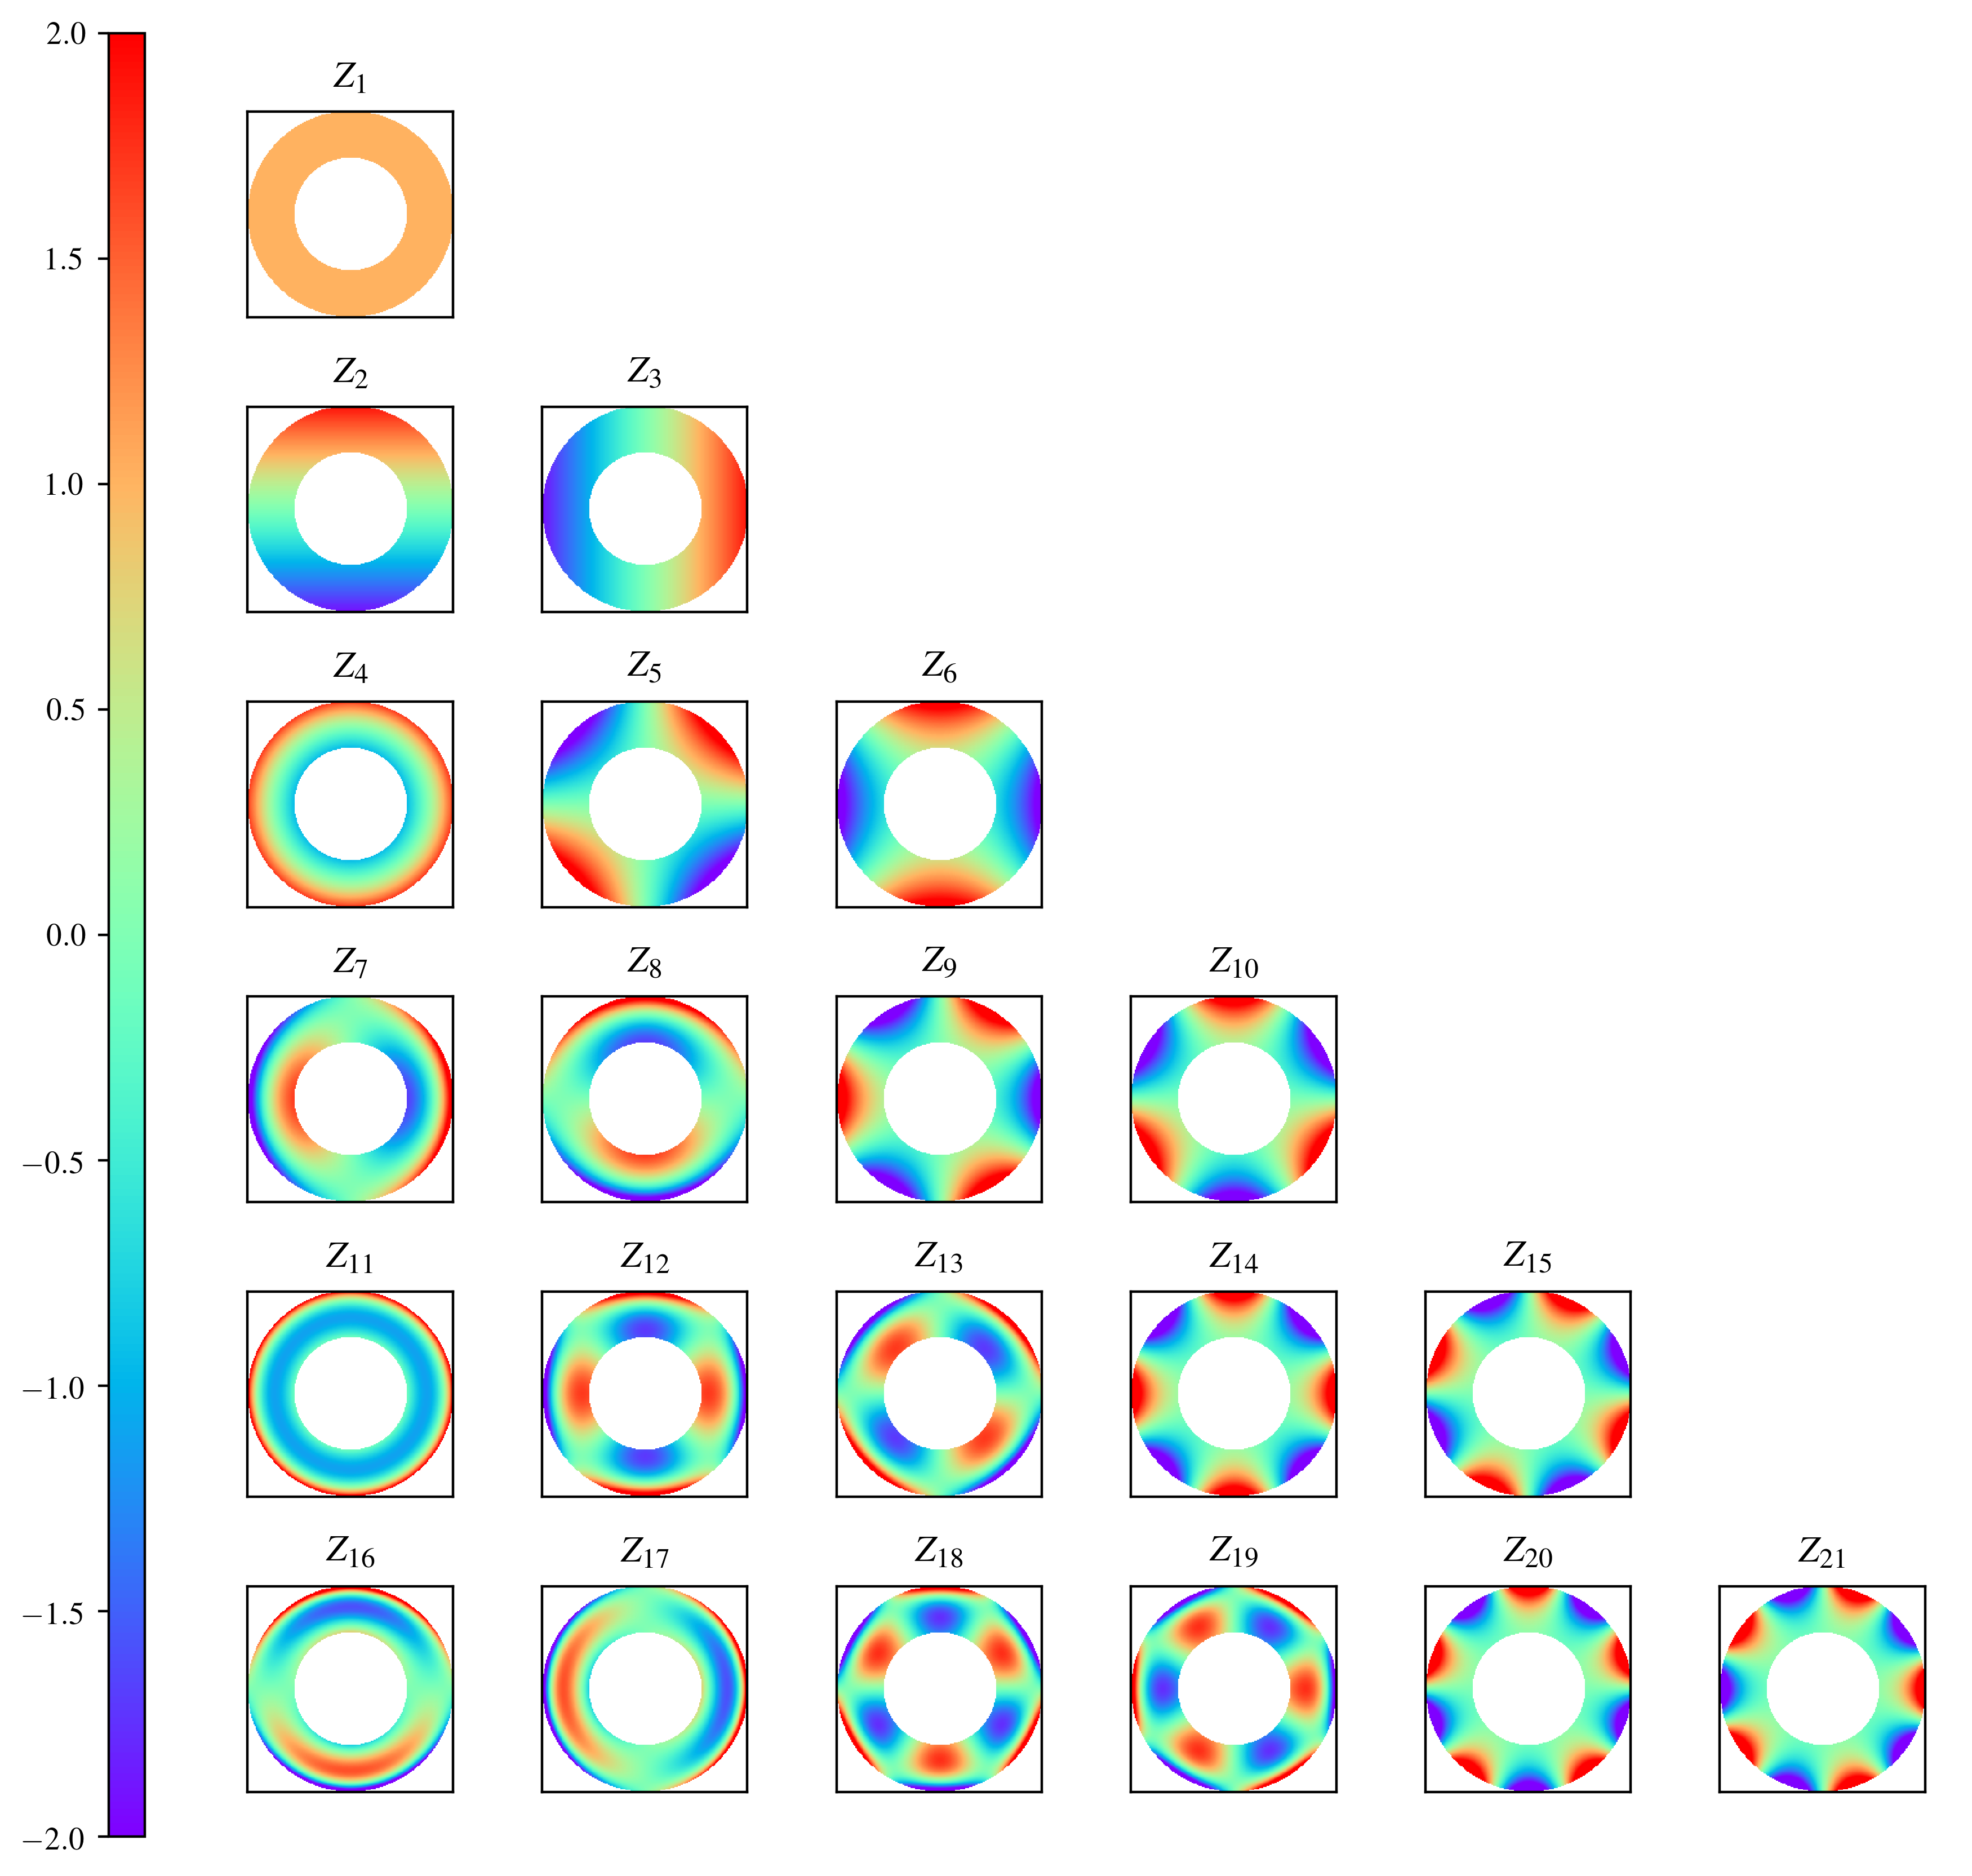
\includegraphics[width=14cm, keepaspectratio]{figs/new_paradigm/zernikes.png}
\caption[Zernike polynomials]{The Zernike polynomials $Z_1$ throught $Z_24$ with the Noll index scheme. The obscuration of the annular domain is consistent with the obscuration in the Rubin optics.}
\label{fig:zernike}
\end{figure}

For small telescopes, this basis can be used to characterize the wavefront in the entrance pupil. For wide-field telescopes like the Rubin Observatory, the wavefront changes non-trivially across the field of view. Thus the wavefront is a four dimensional function of both the entrance pupil and focal plane. One way to model this would be to have another polynomial basis $\{P_i\}$ for the focal plane $x,y$. Then we could write the full wavefront as $W(x,y,\rho, \theta) = \sum_i \sum_j \beta_{ij} P_i(x,y) Z_j(\rho, \theta)$. The coefficients $\beta$ are indexed by the image plane index $i$ and pupil plane index $j$. The double Zernike polynomials are the $P_i(x,y) Z_j(\rho, \theta)$ where the field polynomials are circular Zernike polynomials $P_i = Z_i$ \cite{doublezernike}. Thus $\beta_{ij}$ is the mode of circular polynomial $Z_i$ in the focal plane, and annular polynomial $Z_j$ in the image plane.

In practice we also truncate the focal plane index. This leaves us with a finite set of coefficients to represent the full wavefront across the pupil and focal planes. We found that for the Rubin Observatory, most of the aberration power is concentrated in the first three focal plane polynomials. We simulated 500 perturbed telescope states and numerically calculated the double Zernike coefficients out to index 36. Then we studied the fraction of the aberrated wavefront contained in the first $k$ focal plane Zernikes. We found that the first three polynomials capture 90\% of the wavefront. These first three polynomials are a constant offset, a tip-plane, and a tilt-plane - collectively they define a plane. We suspect a similar pattern holds for other wide field telescopes. It suggests that the 54 double Zernike coefficients $\beta_{ij}$where $1 \leq i \leq 3$ and $4 \leq j \leq 24$ offer a good characterization of the wavefront.

\begin{figure}[hbt!]
\centering
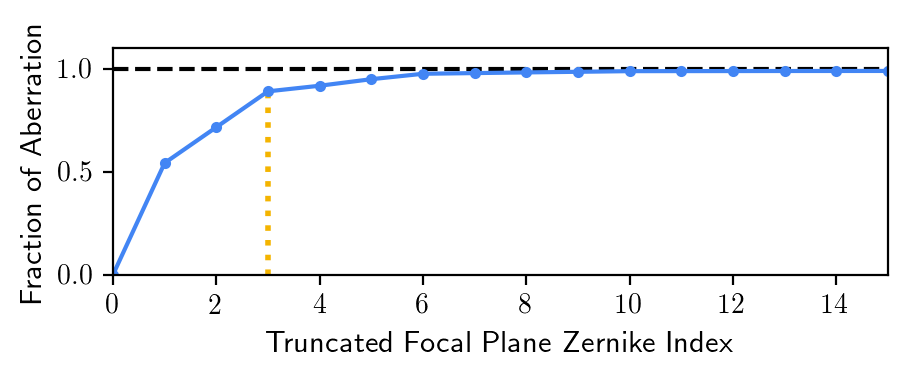
\includegraphics[width=14cm, keepaspectratio]{figs/new_paradigm/truncated.png}
\caption[Aberration Power in Focal Plane Zernikes]{The fraction of the aberration that is present in the first $k$ focal plane Zernike polynomials, where $k$ is the truncation index on the x-axis.}
\label{fig:truncated}
\end{figure}

This separation of the wavefront into pupil and focal plane components is key to this work. Our key insight was as follows. At any point in the image plane, we can use the image to constrain the pupil wavefront at that position - we deem this the \textit{local} wavefront. Then we can interpolate the focal, or \textit{global}, wavefront from all the local estimates. In section \ref{sec:decomposing}, we describe techniques that are very well suited for each of these subproblems. Before then, we summarize recent progress in neural network based phase estimation.

\section{Neural Network Based Phase Estimation}
The potential for neural networks to learn the non-linear mapping between intensity patterns and aberrations in the pupil plane was first recognized in 1990 \cite{1990NatureMLAO}. Shortly afterwards, this potential was realized as neural networks were deployed to detect turbulence induced distortion on the Multiple Mirror Telescope \cite{1991NatureMLAO} and to detect aberrations in the primary mirror of the Hubble Space Telescope \cite{1993HubbleMLAO}. Others expanded this concept to predict more wavefront components \cite{1992SPIE.1706..113J}, incorporate temporal history \cite{1996ESOC...54...95L,1997ApOpt..36..675M}, compare reconstruction methods \cite{2006OExpr..14.6456G}, and better characterize atmospheric turbulence \cite{2008ISTSP...2..624W}. 

In the past decade, convolutional neural networks (CNNs) \cite{726791} have re-emerged and spurred dramatic advances in computer vision \cite{10.5555/2999134.2999257, 10.5555/2999792.2999897, 10.1007/s11263-015-0816-y,7780459}. This has created new possibilities for wavefront sensing in astronomy. In \cite{2018OptL...43.1235P}, the authors created a CNN that could estimate the wavefront from a single PSF image. They used these estimates as initial starting points in a gradient-based optimization and showed this was superior to using random samples. \cite{2019OExpr..27..240N} showed wavefront sensing performance could be improved by introducing a preconditioner to broaden the PSF and create more intensity structure for the neural network to exploit. This brings up interesting new design possibilities for wavefront sensors. While conventional Lyot-based low order wavefront sensing methods have a limited dynamic range due to their linear recovery, \cite{2020OExpr..2826267A} showed that a CNN can extend the aberration range over which the wavefront can be estimated by an order of magnitude.

Previous work on machine learning based wavefront sensing focuses on sensing the full wavefront aberration. Here we focus on sensing the optics wavefront, across the field of view, in the midst of the dominant atmospheric contribution. This problem presents new challenges, such as how to best aggregate intensity information from throughout the field of view to suppress the spatially correlated error due to the turbulence contribution. Our approach is comprised of only two steps, is easy to characterize, and can process each donut image in 6 \textit{milliseconds}.

\section{Wavefront Estimation Framework}
\label{sec:decomposing}

The optics wavefront $W_{\text{opt}}$ is a function of two separate planes: the pupil plane parameterized by $(u,v)$ and the focal plane parameterized by $(x,y)$. We use the double Zernike polynomial basis \cite{doublezernike} to represent the optics wavefront, 
\begin{equation}W_{\text{opt}}(u,v,x,y) = \sum_{i=1}^k\sum_{j=1}^m\beta_{ij}Z_i(u,v)Z_j(x,y)\end{equation}
\noindent where $\beta_{ij}$ are the coefficients, $Z_i$ are annular Zernike polynomials over the pupil, and $Z_j$ are circular Zernike polynomials over the focal plane. The goal of wavefront sensing is to estimate these coefficients $\beta_{ij}$ from the $n$ donut images $D_i$ positioned across the wavefront sensors (see Figure \ref{fig:focalplane}). Let the position of donut $i$ be $x_i,y_i$ and the defocus offset of the corresponding sensor be $z_i$. The wavefront sensing problem is to find $f$ such that
\begin{equation}\beta = f((D_1,x_1, y_1, z_1), \dots, (D_n, x_n, y_n, z_n))\end{equation}

We break this into two subproblems.

\begin{enumerate}
	\item Estimate the local wavefront with a CNN at each donut position.
	\item Interpolate the global wavefront from the local wavefront estimates across the focal plane.
\end{enumerate}

\noindent These steps are outlined in Figure \ref{fig:twostep}. 

\begin{figure}[hbt!]
\centering
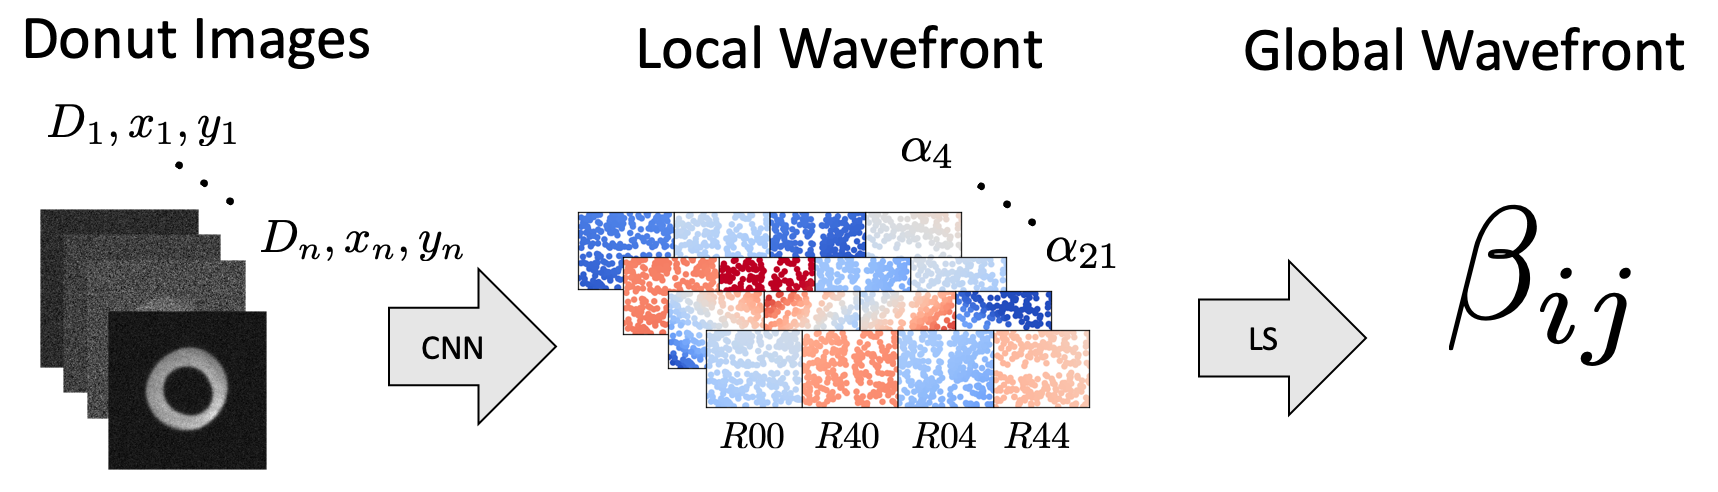
\includegraphics[width=14cm, keepaspectratio]{figs/new_paradigm/twostep.png}
\caption[Two Step Approach To Wavefront Sensing]{In the first step, a convolutional neural network (CNN) processes each donut crop on the four wavefront sensors. In the second step, from each local wavefront coefficient we interpolate three global wavefront coefficients with least squares optimization (LS).}
\label{fig:twostep}
\end{figure}

\subsection{Estimating Local Wavefronts}
In the first subproblem, we estimate the total local wavefront $w_{\text{tot}}(u,v)$ from donut $D_i$ at position $x_i, y_i, z_i$. The intensity in the donut image is related to the total local wavefront by the Fraunhofer diffraction integral (equation \ref{eqn:fraunhofer}). We represent the local wavefront in a basis of annular Zernike polynomials over the pupil, such that the total local wavefront for donut $i$ at position $x_i, y_i$ is
\begin{equation}
w_{\text{tot}}(u,v) = \sum_j \alpha_{ij}Z_j(u,v)
\end{equation}
Convolutional neural networks (CNNs) are particularly well suited for processing images and learning nonlinear mappings. We develop a CNN $\varphi$ to solve the inverse problem of estimating $\alpha_{ij}$ for $j = 1\ \dots m$ from $(D_i,x_i,y_i,z_i)$ . In chapter \ref{chap:cnn} we describe the implementation of this model in detail. 

\subsection{Interpolating the Optics Wavefront}

In the second subproblem, we aggregate the local estimates from the first subproblem to constrain $\beta$. The total local wavefront at position $x_i,y_i$ is related to the optics wavefront via
\begin{equation}w_{\text{tot}}(u,v) = W_{\text{opt}}(u,v|x_i,y_i) + \epsilon(u,v|x_i,y_i)\end{equation}
where $\epsilon$ represents the atmospheric turbulence contribution to the wavefront. Let $\mathcal{Z}$ be defined such that $\mathcal{Z}_{ij} = Z_j(x_i,y_i)$. Then for $i = 1,\dots,m$ we have
\begin{equation}
\alpha e_i = \mathcal{Z} \beta e_i + \epsilon
\end{equation}
where $e_i$ is the $i$th unit vector. Then combining the $\alpha$ from the previous subproblem, and computing the corresponding $\mathcal{Z}$, allows us to solve for $\beta$,
\begin{equation}
\beta = \text{argmin}_{\beta}\left \{\sum_{i=1}^m \ell(\alpha e_i, \mathcal{Z} \beta e_i)\right\}
\end{equation}
where $\ell$ is a convex loss function. Algorithm \ref{alg:main} shows the psuedocode. 

\begin{algorithm}
    % \SetKwInOut{Input}{Input}
    % \SetKwInOut{Output}{Output}
    % \underline{function Estimate Optics Wavefront}\\
    % \Input{combined wavefront sensor image $I \in \mathbb{R}^{N\times N}$}
    % \Output{optics wavefront $\beta \in \mathbb{R}^{k \times m}$}
    \text{given image} $I \in \mathbb{R}^{N \times N}$\\
    \text{initialize local wavefront estimate} $\alpha \in \mathbb{R}^{n \times m}$\\
    \text{initialize global Zernike basis} $\mathcal{Z} \in \mathbb{R}^{n \times k}$\\
    \For{\text{donut} $i$ \text{ in } 1\dots n}
    {
        $D_i = \text{Crop}(I, x_i, y_i)$\\
        $\alpha[i,:] = \varphi(D_i, x_i, y_i, z_i)$\\
        \For{\text{Sernike} $j$ \text{ in } 1\dots k}
        {
        	$\mathcal{Z}[i,j] = Z_j(x_i, y_i)$
        }
    }
    \text{initialize optics wavefront} $\beta \in \mathbb{R}^{k \times m}$\\
    \For{\text{local Zernike } $i$ \text{ in } $1 \dots m$}
    {
      $\beta[:,i] = \text{argmin}_{\beta[:,i]}\ \{\ell(\alpha[:,i], \mathcal{Z}\beta[:,i])\}$\\
    }
    \text{return } $\beta$\\
    \caption{estimates the optics wavefront from donut images.}
    \label{alg:main}
\end{algorithm}

The dominant source of error is the atmospheric turbulence contribution to the wavefront. This error is correlated on scales of arcminutes. By processing donuts with reasonable separation and between different wavefront sensors we are able to suppress this error by roughly a factor of $1 / \sqrt{n}$ where $n$ is the number of donuts used.

There are two parameters of our algorithm that must be set based on the telescope: the number of Zernike coefficients to use for the pupil $m$, and the number of Zernike coefficients to use for the focal plane $k$. For the Rubin Observatory we use Zernikes $Z_4$ through $Z_{21}$ for the pupil plane. The first three coefficients do not impact image quality, so we exclude them. We truncate the basis at $Z_{21}$, a convention set by \cite{2015Xin}, as the higher order terms have very small coefficients in practice. We use $Z_1$ through $Z_3$ for the focal plane. Our simulations show that 90\% of the optics wavefront is contained in this truncated basis.

There are two benefits to dividing the wavefront estimation problem into these two subproblems that are worth highlighting. The first is the useful intermediate data products. The local wavefront coefficients $\alpha$, which are estimated in the first subproblem, are physically meaningful. Telescope operators can track them during operations and gain further insight into the system. This adds an additional layer of transparency and robustness.

The second benefit is that it makes deep learning approaches feasible. Deep neural networks must be trained on large datasets to avoid overfitting. The input to the original problem is four wavefront sensor images, or up to thousands of donut images. The raytracing necessary to simulate even a single input sample is computationally expensive. In our first subproblem however, the input is only a single donut image. This reduces the computation required to produce a training sample by three orders of magnitude and makes it possible to generate simulated datasets that are sufficient for training deep neural networks. In chapter \ref{chap:cnn}, we highlight the power of these models.


% Full title as you would like it to appear on the page
\chapter{The Rubin Observatory Active Optics System}
\label{chap:aos}
% Short title that appears in the header of pages within the chapter
\chaptermark{Rubin Active Optics}

\epigraph{Some people don't like change, but you need to embrace change if the alternative is disaster.}{Elon Musk}

\section{Rubin Telescope}
The Vera C. Rubin Observatory is a 8.4-m wide-field telescope designed to measure the structure and evolution of the universe. The roots of the observatory date back twenty years ago to a 2001 proposal for The Dark Matter Telescope \cite{2001ASPC..237..417T}. The original scientific motivation was to produce premier weak lensing catalogs. Since then, the facility has gone through two name changes (it was the Large Synoptic Survey Telescope for many years) and the purview has expanded to include cataloging the solar system, mapping the milky way, and exploring the transient and variable sky \cite{sciencebook}. Site construction began on Cerro Pach\'{o}n, Chile in 2015 and is expected to be completed in 2023 \cite{2020SPIE11445E..0IT, 2020SPIE11445E..1US}. 

Rubin will have a $319\ \text{meter}^2\text{degrees}^2$ \'{e}tendue, ten times larger than any previous or currently planned telescope. The large \'{e}tendue is achieved by a novel three mirror design with a very fast f/1.234 beam. The design is optimized to attain seeing limited image quality across the $9.6\ \text{deg}^2$ field of view and passband spanning $320-1050\ nm$. Figure \ref{fig:telescope} shows the light path through the optics. The incident light first strikes the annular primary mirror M1, which has an outer diameter of $8.4\ m$ and an effective filled aperture of $6.4\ m$. Next the light visits the $3.4\ m$ convex secondary mirror M2 and the $5.0\ m$ concave tertiary mirror M3. Then the light passes through three refractive camera lenses and onto the $64\ cm$ focal plane. 

The primary and tertiary mirrors, M1 and M3, share an inner and outer radius respectively. This was chosen so that they could be fabricated from a single monolithic blank using spin-cast borosilicated technology. We refer to this collective mirror as M1M3. 

\begin{figure}[hbt!]
\centering
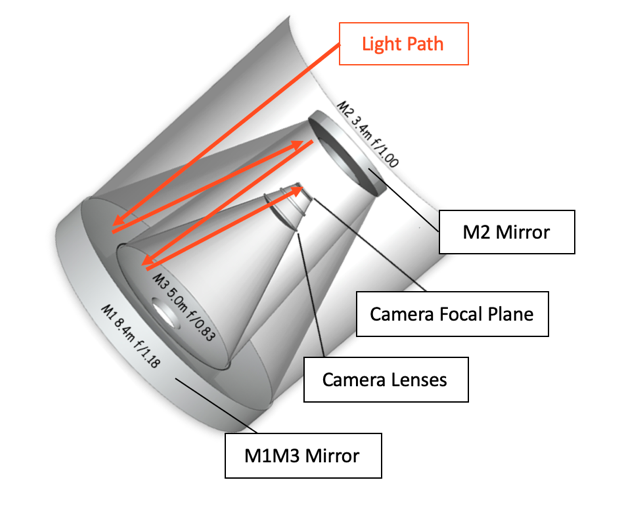
\includegraphics[width=14cm, keepaspectratio]{figs/rubin_telescope_and_aos/telescope.png}
\caption[Rubin Optics]{The optic elements of the Rubin telescope. The light path through the optics is shown in orange.}
\label{fig:telescope}
\end{figure}

\section{Active Control}

There are two telescope properties that incentivize the creation of telescopes with large primary mirrors. First, the \'{e}tendue, or light collecting power of a telescope is proportional to the area of the primary mirror. Second, the diffraction limited seeing is inversely proportional to the diameter of the primary mirror. Historically these primary mirrors were thick in order to maintain their nominal surface figure. However, the maximum size possible by these manufacturing processes is 5-6 meters of diameter.

In the late 1980s active optics technology was developed to enable the construction of a generation of telescopes with 8 meter primary mirrors. The mirrors for telescopes with this technology are thin and malleable. For Rubin, the mirrors are made out of borosilicate, which also quickly equilibrates with the ambient temperature. Active optics works by actively adjusting degrees of freedom of the telescope, including the mirror surface, based on a feedback system. The main sources of deviation to correct for are mechanical stresses stemming from the dyamics, wind, and gravity and temperature gradients in the mirror surfaces.

Figure \ref{fig:m1m3act} shows the active components of the combined primary and tertiary mirrors M1M3. The position in the x,y, and z directions is controlled by six large actuator hardpoints that form a hexapod. The mirror surface is controlled by 156 pnuematic actuators. The distribution of the actuators and their axes is explained in detail in \cite{2016SPIE.9906E..0QN}, although these details are not critical for this thesis. Given that even the large hardpoint acutators are pneumatic it is apt to say that the mirror sits on air. 

\begin{figure}[hbt!]
\centering
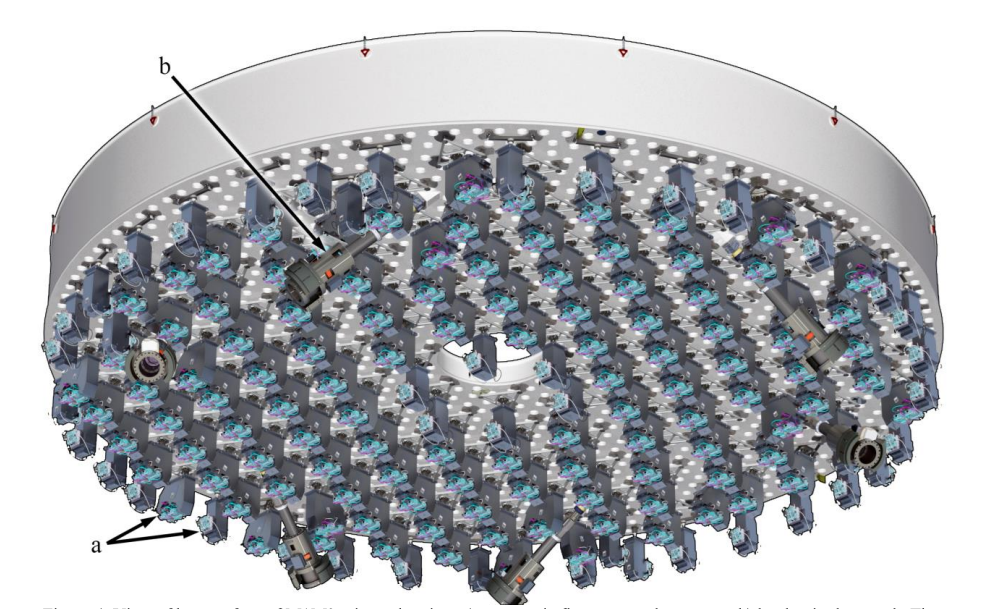
\includegraphics[width=14cm, keepaspectratio]{figs/rubin_telescope_and_aos/M1M3actuators.png}
\caption[Rubin M1M3 Hexapod and Pneumatic Actuators]{View of the bottom face of the M1M3 mirror showing: (a) pneumatic figure control actuators and (b) hard point hexapod. Source: \cite{2016SPIE.9906E..0QN}.}
\label{fig:m1m3act}
\end{figure}

Figure \ref{fig:m2act} shows the active components of the aspherical secondary mirror M2. The position in the x,y, and z directions is controlled by six large tangential electromechanical actuators. The mirror surface is controlled by 72 axial electromechanical actuators. The details of the configuration, metrology, and testing are described further in \cite{2016SPIE.9906E..67N}. Again, these details are not strictly necessary for what follows.

\begin{figure}[hbt!]
\centering
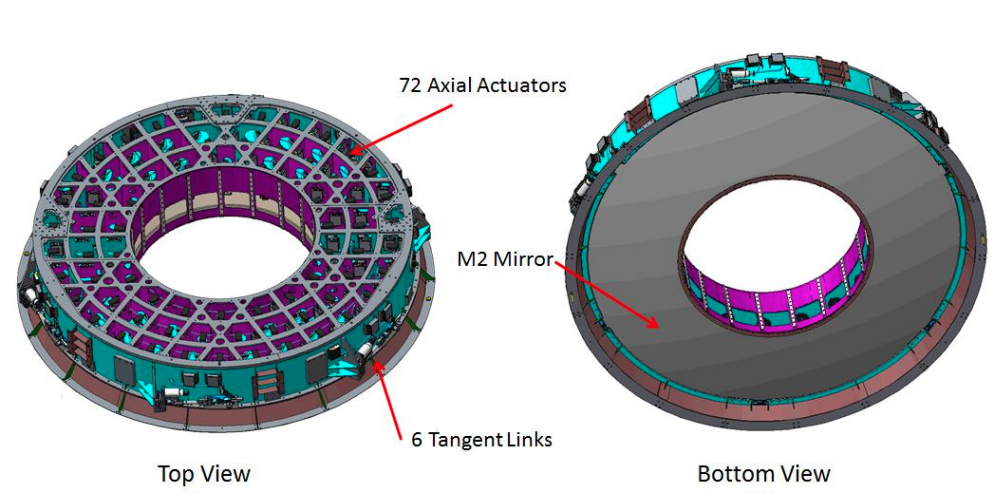
\includegraphics[width=14cm, keepaspectratio]{figs/rubin_telescope_and_aos/M2actuators.png}
\caption[Rubin M2 Hexapod and Mechanical Actuators]{Top and bottom views of the secondary mirror M2 showing the mirror cell, mirror, axial actuators, and tangential hard points. Source: \cite{2016SPIE.9906E..67N}.}
\label{fig:m2act}
\end{figure}

While it is important to understand the underlying physical interfaces for controlling the telescope, we use a key abstraction to reduce the dimensionality of the problem. Instead of modeling the state of the mirror surfaces with hundreds of predicted actuator deviations, we use low order bending modes. These are the modes that are most excited by the aforementioned sources of perturbations. Not only does this allow us to reduce the dimensionality by an order of magnitude, it also better captures the deviations we care about. We use finite element simulations to determine which modes have the most power and how many modes are required to maintain Rubin image quality specifications. 

At the time this work was initiated, all the bending modes had not been confirmed. Thus we decided to parameterize deviations to the mirror surface with the first 20 annular Zernike polynomials. We do not belive this choice has significant impact on the analysis. Table \ref{tab:dof} shows the 50 degrees of freedom - 5 for each hexapod and 20 for each mirror surface. It is worth emphasizing that this telescope's predecessor, the Dark Energy Camera on the Blanco Telescope, only controls 8 degrees of freedom. 

\begin{table}[hbt!]
\caption[The 50 Telescope Degrees of Freedom]{\label{tab:dof}The 50 telescope optics control parameters. Notation: dx is a translation in the x-axis and rx is a rotation along the x-axis.} 
\begin{center}
\begin{tabular}{|l|l|}
\hline
\rule[-1ex]{0pt}{3.5ex} Camera hardpoints & dx, dy, dz, rx, ry \\
\hline
\rule[-1ex]{0pt}{3.5ex} M2 hardpoints & dx, dy, dz, rx, ry \\
\hline
\rule[-1ex]{0pt}{3.5ex} M1M3 figure & 20 surface bending modes \\
\hline
\rule[-1ex]{0pt}{3.5ex} M2 figure & 20 surface bending modes \\
\hline
\end{tabular}
\end{center}
\end{table} 

\section{Wavefront Sensors and Donut Images}

In the last section we discussed the degrees of freedom we are trying to predict and control. In this section we describe the feedback system that makes this possible. 

The Rubin focal plane is comprised of 189 science sensors, 4 wavefront sensors, and 8 guidestar sensors \cite{10.1117/12.926710}. The wavefront sensors, in the four corners of the focal plane, are used for active optics. Each $4k\ \times\ 4k$ pixel sensor consists of two $2k\ \times 4k$ pixel half-chips. One half-chip is $1.5\ mm$ intra-focal; the other is $1.5\ mm$ extra-focal. The stars on these images are called \textit{donuts} because of their annular, donut-like shape. Figure \ref{fig:focalplane} shows the layout of the focal plane and simulated donut images.

\begin{figure}[hbt!]
\centering
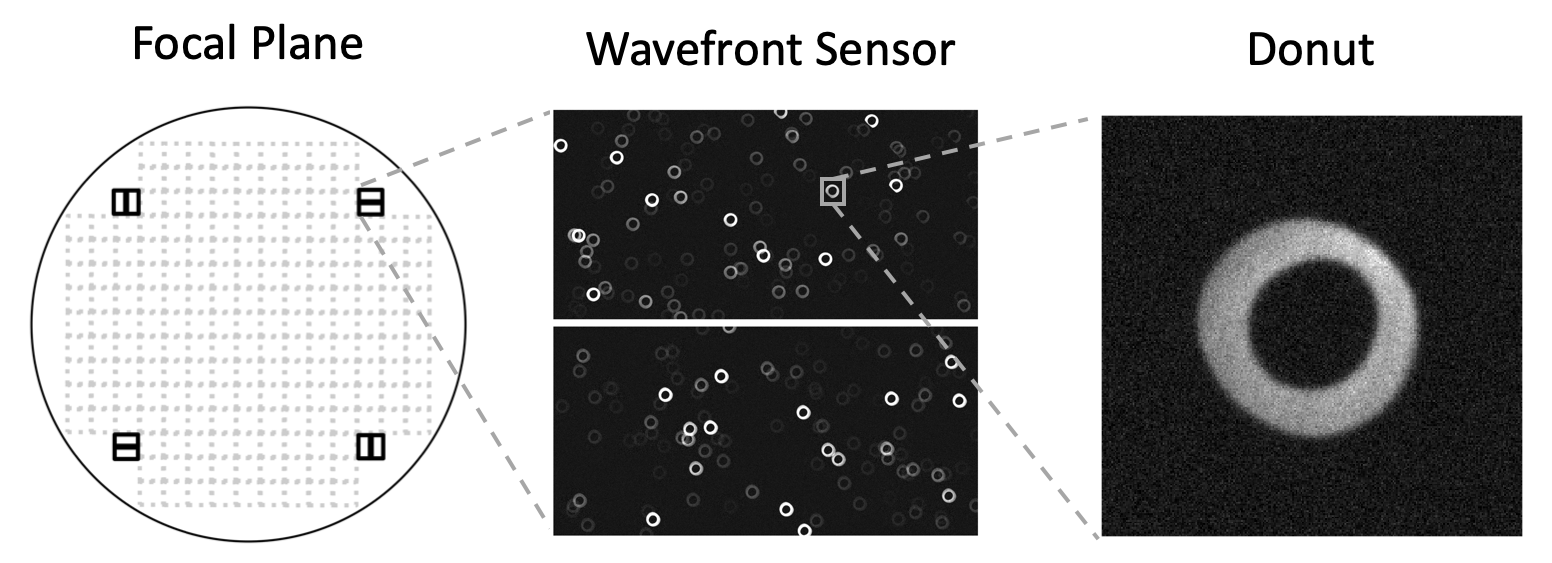
\includegraphics[width=14cm, keepaspectratio]{figs/rubin_telescope_and_aos/wavefrontsensorbreakdown.png}
\caption[From Focal Plane, To Wavefront Sensor, To Donut Image]{Left: the Rubin focal plane; science sensors are in gray; wavefront sensors are in black. Middle: One wavefront sensor split into intra-focal and extra-focal half-chips. Right: a single $256\ \times\ 256$ pixel crop of a donut.}
\label{fig:focalplane}
\end{figure}

The annular shape of the donut image stems from the outline of the M1 aperature. Figure \ref{fig:focalplane} highlights this intuition. The intra-focal and extra-focal sensors cut off the Rubin beam before it has converged. The intensity pattern in these larger images provide more information about the location of perturbations that are accounted for across the entrance pupil.

\begin{figure}[hbt!]
\centering
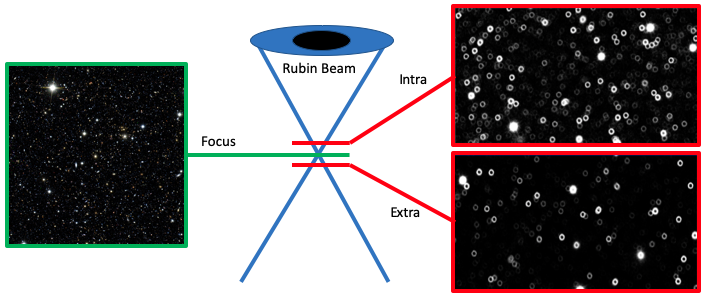
\includegraphics[width=14cm, keepaspectratio]{figs/rubin_telescope_and_aos/donutintuition.png}
\caption[Donut Image Intuition]{The images formed from placing sensors at different positions along the optical path. The optical path from the pupil to focus is shown in blue. The image produced at focus is shown in green. The intra-focal and extra-focal images are shown in red. The donut shape stems from the annular entrance pupil.}
\label{fig:focalplane}
\end{figure}



\chapter{Simulating High Fidelity Rubin Donut Images}
\label{chap:sim}
\chaptermark{Simulating Donut Images}

% \epigraph{The first principle is that you must not fool yourself and you are the easiest person to fool.}{Richard Feynman}

\epigraph{Perhaps one day we will have machines that can cope with approximate task descriptions, but in the meantime, we have to be very prissy about how we tell computers to do things.}{Richard Feynman}

Simulation is a cornerstone of this work. The Rubin Observatory is not complete, which in some sense necessitates using simulated data. However, even if the observatory was complete and we could collect real data, it would still be challenging to adequately sample the 50 dimensional state space of the telescope. In real life, to configure the Rubin telescope in a perturbed state takes on the order of 10 seconds. In code, initializing a telescope instance in a specific configuration takes single digit microseconds. In real life, there is only one telescope, whereas using the Sherlock cluster at Stanford University, we can initialize the telescope in up to roughly one thousand parallel processes. In short, we exploit simulation to create richer datasets to train and assess our framework.

In the first section, we describe the details of simulating a single donut. In the following sections, we describe the two datasets used in this work. 

\section{Simulating A Single Donut Image}

We use high fidelity Rubin Observatory image simulations to train our model and analyze its performance. By selecting different observational, atmospheric, and telescope parameters for each donut, we produced a simulated training dataset that spans a wide variety of conditions. The output of each simulation $i$ is a $256 \times 256$ pixel donut image $D_i$, and the corresponding true local wavefront $\alpha_i \in \mathbb{R}^{18}$. Figure \ref{fig:donut} shows an example pair of end products. 
% 
\begin{figure} [!htbp]
\begin{center}
\begin{tabular}{c}
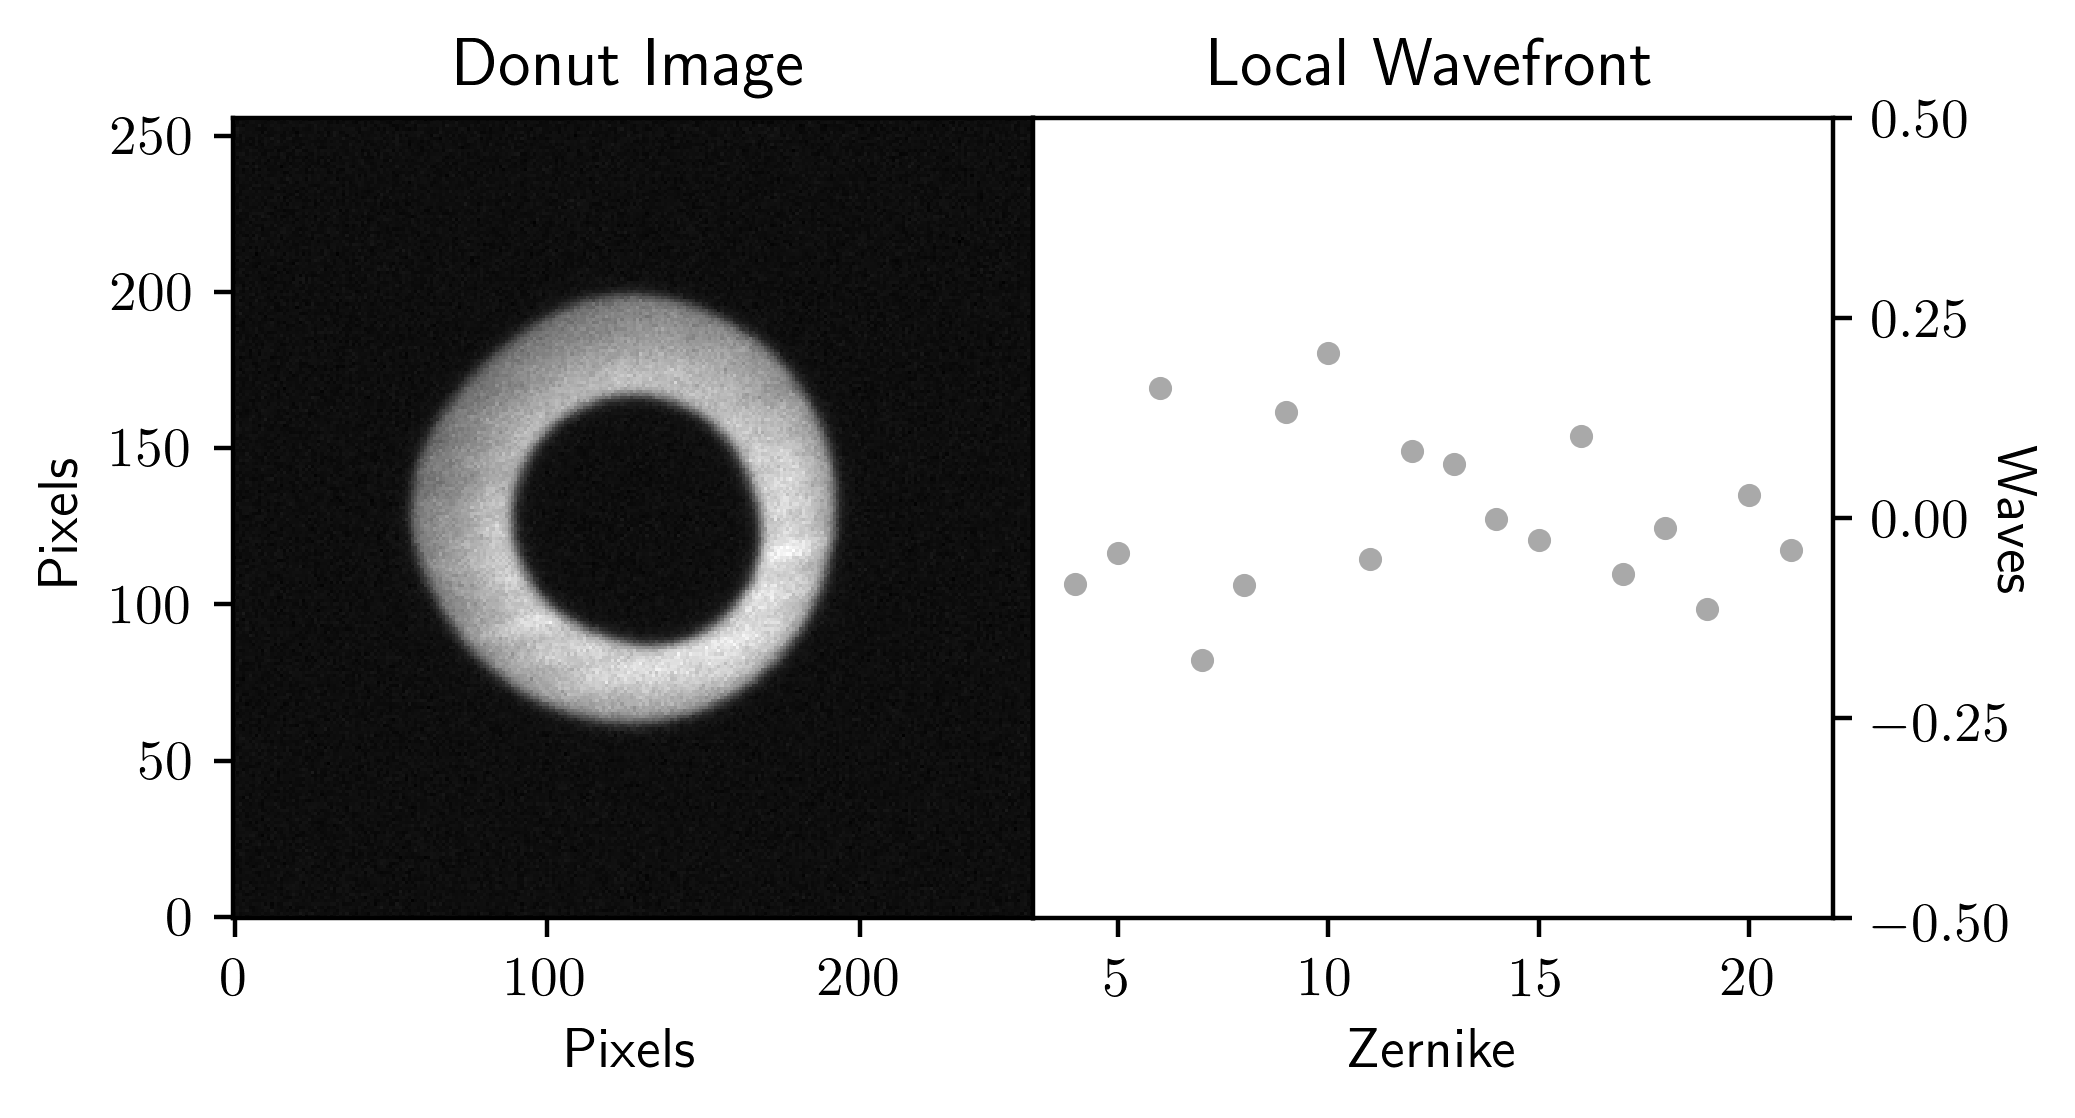
\includegraphics[width=6in]{figs/simulating_donuts/example_atm.png}
\end{tabular}
\end{center}
\caption[Simuated Donut and Local Wavefront]{\textit{Left:} a simulated $256\ \times\ 256$ pixel donut image at the $(x,y)$ field position ($-1.1048^o$, $1.0868^o$). \textit{Right:} the corresponding local wavefront annular Zernike coefficients ($Z_4-Z_{21}$ inclusive), measured in units of 622.20 nm waves. \label{fig:donut}}
\end{figure}

\begin{figure} [!htbp]
\begin{center}
\begin{tabular}{c}
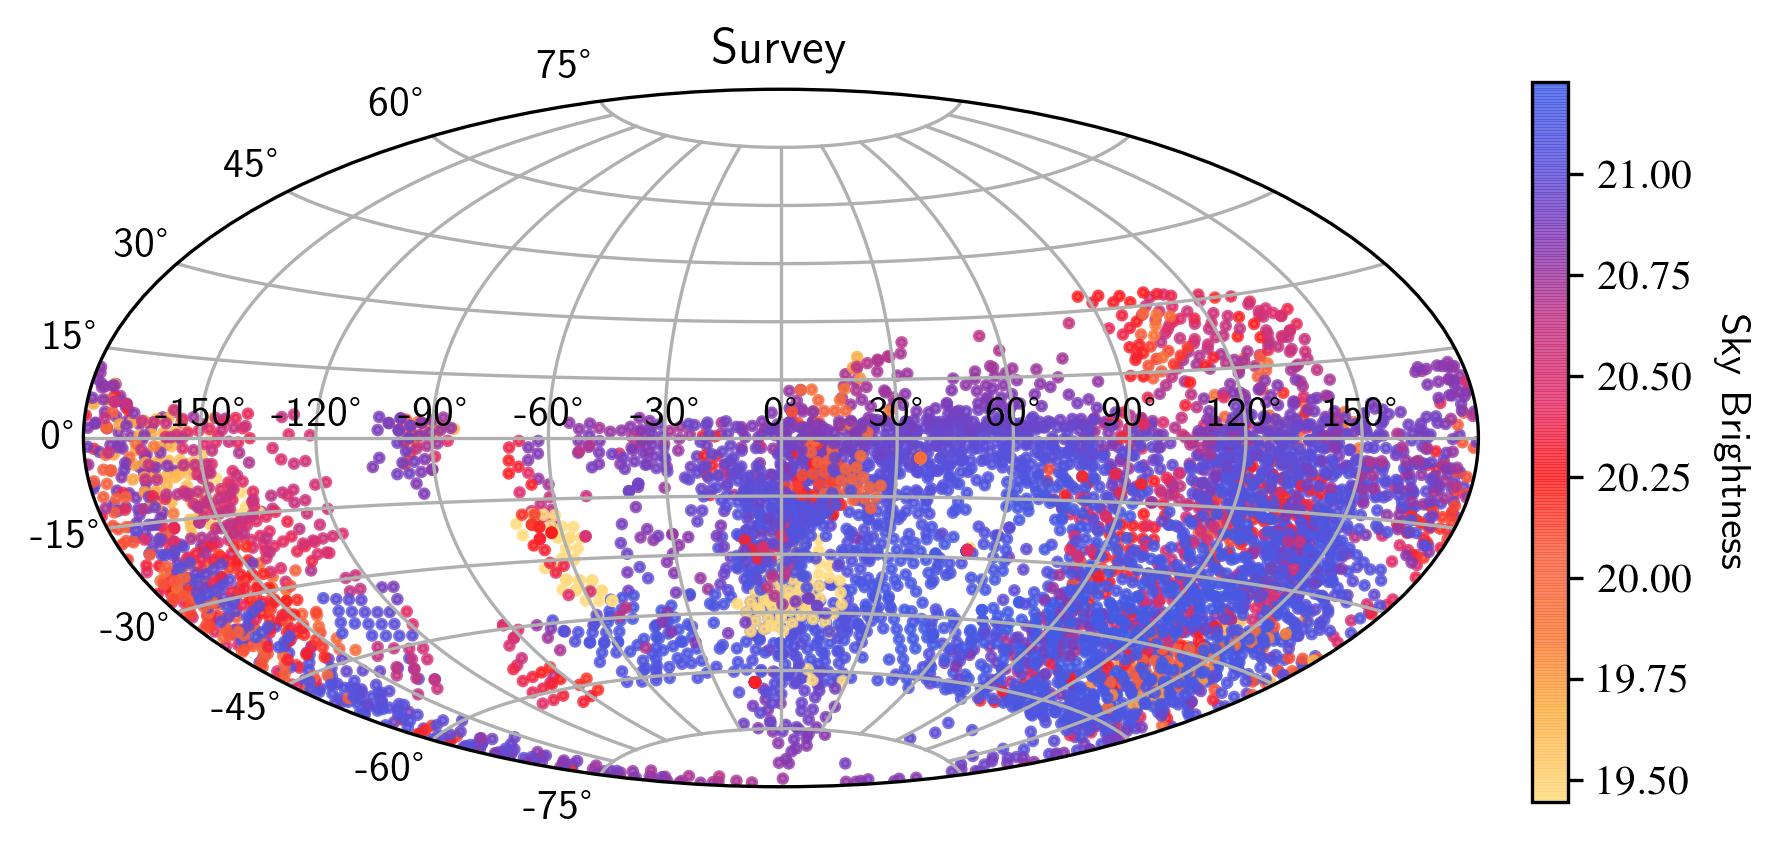
\includegraphics[width=6in]{figs/simulating_donuts/survey.png}
\end{tabular}
\end{center}
\caption[Survey Footprint]{The right ascension and declination of the observations we use for our simulations. Each point corresponds to an observation; the color shows the variation in sky brightness.\label{fig:survey}}
\end{figure}

The simulations are comprised of sequential steps that trace a photon's journey from a distant source to a count in a pixel in an image. The first step is to generate photons in the sky corresponding to a source from the observation. We create a baseline survey to draw observations from. The survey is comprised of 5497 randomly drawn r-band visits from the Operations Simulator (OpSim) \cite{opsim}. Figure \ref{fig:survey} shows the distribution of the observations across the sky. This survey samples a wide range of sky brightnesses, atmospheric seeing, and sky positions. 

For each of these visits, we determine the fields of view covered by the four corner wavefront sensors. Then we query the Gaia DR2 catalog for sources within these regions and with G magnitudes less than 18 \cite{dr2}. The mean number of sources per catalog is $1101$ with a standard deviation of $1720$. The largest catalog contains $12684$ sources. Once we have the catalog, we convert the Gaia $G$, $G_{bp}$, and $G_{rp}$ magnitudes to the SDSS $r$ magnitude based on Equation \ref{eqn:conversion} from the Gaia data release documentation \cite{conversion}.

\begin{align}\label{eqn:conversion}
x &= G_{bp} - G_{rp}\\
r &= G + 0.12879 - 0.24662 \cdot x + 0.027464 \cdot x^2 + 0.049465 \cdot x^3
\end{align}

\noindent We clip SDSS $r$ magnitudes below 14 to save simulation time. The simulation starts by selecting a source and generating the corresponding photons. The number of photons is determined by the SDSS magnitude and the wavelengths are drawn from a black body distribution with spectral radiance,

\begin{equation}\label{eqn:blackbody}
B(\lambda, T) = \frac{2hc^2}{\lambda^5}\frac{1}{e^{\frac{hc}{\lambda k_B T}} - 1}
\end{equation}

\noindent based on the temperature of the source. After the photons are generated, the next stage of simulation propagates them through the atmosphere.

The primary contribution from the atmosphere is atmospheric turbulence. We use the GalSim Python package to split the atmospheric turbulence power spectrum into low and high spatial frequencies and simulate their contribution separately \cite{galsim}. The low spatial frequencies modulate the centroid of the source photons. The high spatial frequencies scatter the photons around this centroid, sometimes called the \textit{second kick} \cite{phosim}. The phase screens are initialized with altitudes and velocities from atmospheric tomography profiles \cite{atmosphere}. The Fried parameter for the atmosphere is determined by the airmass and seeing from the OpSim observation and by the central wavelength of the $r$ bandpass, $622.20\ nm$. 

In addition to the turbulence contribution, we also incorporate chromatic seeing and differential chromatic refraction \cite{chromatic}. Both of these are functions of the wavelengths of individual photons. We model chromatic seeing by scaling the turbulence induced perturbations based on wavelength. We model chromatic refraction by refracting the photons along the meridian based on the airmass. At the conclusion of this step, there is a bundle of photons at the entrance pupil of the telescope.

Next, we trace photons from the entrance pupil of the primary mirror to the plane of the detector. The batoid Python package was used to construct model Rubin telescope instances and perform the ray tracing \cite{batoid}. We constructed telescope instances that have 50 degrees of freedom that are analogous to those in Table \ref{tab:dof}. For simplicity, we used 20 Zernike polynomials ($Z_4 - Z_{23}$) to represent the surface bending modes. We skip the first three Zernike modes because these surface perturbations would be degenerate with the hardpoint control parameters.

In order to determine a reasonable range for the degrees of freedom, we first computed the single parameter excitation levels, shown in Table \ref{tab:range}, that induce the global wavefront to have root-mean-square error of 0.3 wavelengths, or \textit{waves}. We set the amplitude of a given parameter by drawing from a normal distribution that is centered on the center of the range and has a standard deviation of half the range multiplied by $\sqrt{5/50}$. This means that the total error across all the control parameters will be roughly 5 times the error that on an individual parameter would make the global wavefront 0.3 waves (where a wave is the central wavelength of the r bandpass, or 622.20 nm).

\begin{table}[!htbp]
\caption[Range of Simulated Control Parameters]{\label{tab:range}The range in each degree of freedom where the root-mean-square of the global wavefront is below 0.3 waves (one wave is 622.20 nm). These ranges are used to create realistically deformed telescope instances in our simulations. Notation: dx is a translation in the x-axis; rx is a rotation along the x-axis; $Z_4$ is the fourth annular Zernike polynomial over the annulus of the corresponding surface.} 
\begin{center}
% \small
\begin{tabular}{|l|c|c|l|c|c|r|}
\hline
Parameter & Min & Max & Parameter & Min & Max\\
\hline
Camera dx \hfill (um) & -580 & 580 & M2 dx \hfill (um) & -118 & 118 \\
Camera dy \hfill (um) & -580 & 580 & M2 dy \hfill (um) & -118 & 118 \\
Camera dz \hfill (um) & -10.7 & 5.39 & M2 dz \hfill (um) & -11.1 & 11.1 \\
Camera rx \hfill (urad) & -42.0 & 42.0 & M2 rx \hfill (urad)& -17.6 & 17.6 \\
Camera ry \hfill (urad) & -42.0 & 42.0 & M2 ry \hfill (urad) & -17.6 & 17.6 \\
M1M3 $Z_4 $\hfill (nm) & -111 & 56.4 & M2 $Z_4 $ \hfill (nm) & -59.1 & 117 \\
M1M3 $Z_5 $\hfill (nm) & -42.4 & 42.4 & M2 $Z_5 $ \hfill (nm) & -68.9 & 68.9 \\
M1M3 $Z_6 $\hfill (nm) & -42.4 & 42.4 & M2 $Z_6 $ \hfill (nm) & -68.9 & 68.9 \\
M1M3 $Z_7 $\hfill (nm) & -65.0 & 65.0 & M2 $Z_7 $ \hfill (nm) & -76.4 & 76.4 \\
M1M3 $Z_8 $\hfill (nm) & -65.0 & 65.0 & M2 $Z_8 $ \hfill (nm) & -76.4 & 76.4 \\
M1M3 $Z_9 $\hfill (nm) & -45.9 & 45.9 & M2 $Z_9 $ \hfill (nm) & -70.6 & 70.6 \\
M1M3 $Z_{10}$ \hfill (nm) & -45.9 & 45.9 & M2 $Z_{10} $ \hfill (nm) & -70.6 & 70.6 \\
M1M3 $Z_{11}$ \hfill (nm) & -130 & 66.2 & M2 $Z_{11} $ \hfill (nm) & -62.8 & 70.4 \\
M1M3 $Z_{12}$ \hfill (nm) & -51.5 & 51.5 & M2 $Z_{12}$ \hfill (nm) & -68.3 & 68.3 \\
M1M3 $Z_{13}$ \hfill (nm) & -51.5 & 51.5 & M2 $Z_{13}$ \hfill (nm) & -68.3 & 68.3 \\
M1M3 $Z_{14}$ \hfill (nm) & -48.1 & 48.1 & M2 $Z_{14}$ \hfill (nm) & -73.6 & 73.6 \\
M1M3 $Z_{15}$ \hfill (nm) & -48.1 & 48.1 & M2 $Z_{15}$ \hfill (nm) & -73.6 & 73.6 \\
M1M3 $Z_{16}$ \hfill (nm) & -73.6 & 73.6 & M2 $Z_{16}$ \hfill (nm) & -68.0 & 68.0 \\
M1M3 $Z_{17}$ \hfill (nm) & -73.6 & 73.6 & M2 $Z_{17}$ \hfill (nm) & -68.0 & 68.0 \\
M1M3 $Z_{18}$ \hfill (nm) & -49.7 & 49.7 & M2 $Z_{18}$ \hfill (nm) & -64.8 & 64.8 \\
M1M3 $Z_{19}$ \hfill (nm) & -49.7 & 49.7 & M2 $Z_{19}$ \hfill (nm) & -64.8 & 64.8 \\
M1M3 $Z_{20}$ \hfill (nm) & -49.2 & 49.2 & M2 $Z_{20}$ \hfill (nm) & -76.5 & 76.5 \\
M1M3 $Z_{21}$ \hfill (nm) & -49.2 & 49.2 & M2 $Z_{21}$ \hfill (nm) & -76.5 & 76.5 \\
M1M3 $Z_{22}$ \hfill (nm) & -67.7 & 51.5 & M2 $Z_{22}$ \hfill (nm) & -59.0 & 57.2 \\
M1M3 $Z_{23}$ \hfill (nm) & -51.3 & 51.3 & M2 $Z_{23}$ \hfill (nm) & -65.7 & 65.7 \\
\hline
\end{tabular}
\end{center}
\end{table} 

Once the photons are at the detector, we simulate sensor effects. We use GalSim to simulate the aggregation of photons into silicon pixels. The silicon model includes electron diffusion to account for the nonlinear brighter-fatter effect \cite{brighterfatter}. We also use GalSim to introduce shot noise from the sky background and simulate the camera readout. Then we zero both individual pixels and columns following sensor statistics taken in the lab. At this point, we have a $256 \times 256$ pixel digital image of counts like the one shown in Figure \ref{fig:donut}.

For each donut image, we also simulate the corresponding local wavefront. We use the Batoid package to compute the wavefront at the donut's field position $x,y$. The local wavefront $\alpha$ is represented by the 18 annular Zernike coefficients which have the largest impact on image quality ($Z_4 - Z_{21}$ inclusive). These coefficients serve as the labels for the neural network described in the next Chapter.

In addition to donuts from individual stars, we also simulated blended donuts. These arise when the donut images from two or more stars overlap. In these simulations, the photons from all the overlapping stars are aggregated on the sensor, then the sensor effects are simulated once. In crowded fields, the majority of the donuts will be blends. This data helps us assess this scenario and the density limits of the fields where we can successfully apply our algorithm. 

In the next two Sections we describe the datasets used to train the neural network and to test the full framework, respectively.

% We believe these simulations capture the core attributes of individual donut images and their corresponding wavefronts. There are two ways we can make these simulations more holistic in future work. The first is to include blending from overlapping donuts. In this work, we process each donut individually, whereas in real operation we expect many of the donuts to be blended. The second is using multiple bands. All the analysis in this work is done on images from the r-band. We believe that after demonstrating the efficacy of this technique in the r band, we will be able to easily extend the model to the other bands with transfer learning.

\section{Donut Dataset}

The donut dataset consists of samples with three components: the simulated donut image $D$, the focal plane position $r$ - which includes distance along the focal $z$ axis, and the true local wavefront $\alpha$. The dataset is used to train, validate, and test models for the task,

\begin{equation}\label{eqn:blackbody}
(D,r) \to \alpha
\end{equation}

Modern neural networks, like the one we develop in Chapter \ref{chap:cnn}, typically have millions of parameters. In order to constrain these parameters and simultaneously avoid overfitting, these models must be trained on copious amounts of data. 

For each of the first 5,000 visits from the observing schedule, we simulate 200 individual donut images. The most computationally expensive part of these simulations is generating the atmospheric phase screens. We speed up the simulations by using one atmosphere for every 100 donuts. Telescope instantiation, on the other hand, costs a few microseconds, so we draw a different 50-dimensional perturbation to the nominal telescope state for each donut image. We also simulate 100,147 blends from the same observations. 

Following the standard machine learning cross validation paradigm, we break this data up into training, validation, and test segments. The training, validation, and test sets are comprised of 498,071 stars and 100,028 blends, 220 stars and 36 blends, and 1,708 stars and 340 blends respectively. Figure \ref{fig:donutbox} shows 100 example donuts from the training set. 

\begin{figure} [!htbp]
\begin{center}
\begin{tabular}{c}
\includegraphics[width=\textwidth]{figs/simulating_donuts/huge_donut_box.png}
\end{tabular}
\end{center}
\caption[Example Donuts from Donut Dataset]{Example donuts from the training set. The different degrees of vignetting, missing columns, blending, and turbulence can be seen with the naked eye.\label{fig:donutbox}}
\end{figure}

\section{Full Visit Dataset}

The full problem involves going from $n$ donut images and positions to the 54 coefficients $\beta$,

\begin{equation}\label{eqn:blackbody}
(D_1,r_1), \dots, (D_n, r_n) \to \alpha_1, \dots, \alpha_n \to \beta
\end{equation}

\noindent In addition to the donut dataset, we also need a dataset of full visits, where each visit contains many donut images, so that we can assess how well our framework predicts $\beta$.

Each sample in this dataset consists of all the donut images and positions in the observation, plus the full optics wavefront $\beta$. We used the last 497 observations from the scheduler simulations for the observations. For each visit, we simulated all the stars, and blends, from the Gaia catalog that fall on the corner wavefront sensors. The mean, median, and maximum number of sources in a sample is 787, 222, and 4,998 respectively. Figure \ref{fig:sensordonut} shows an example sample.

\begin{figure} [!htbp]
\begin{center}
\begin{tabular}{c}
\includegraphics[width=\textwidth]{figs/simulating_donuts/sensors_and_donuts.png}
\end{tabular}
\end{center}
\caption[Example Full Visit Sample]{The eight wavefront sensor half-chips in an example sample from the full visit dataset. This sample contains 1112 donut images which are highlighted in blue boxes. \label{fig:sensordonut}}
\end{figure}

All the donuts within a single observation are simulated with the same atmosphere and sky background. Otherwise, each star in the observation is simulated in the same manner as the donuts dataset described above. For each observation, we used the batoid framework to compute the optics wavefront double Zernike coefficients for the perturbed telescope instance.

The largest difference between observations is the density of sources in the field. The number of sources in a sample ranges from 111 to 4998. On average, 32 percent of the sources are blends. However, for the crowded fields this number can be over 90 percent. Figure \ref{fig:blendfraction} shows how the fraction of sources that are blends increases with the total number of sources in the visit. Thus, while for less crowded fields ample un-blended stars are available, for crowded fields, the wavefront sensing algorithm's ability to process blends is critical.

\begin{figure} [!htbp]
\begin{center}
\begin{tabular}{c}
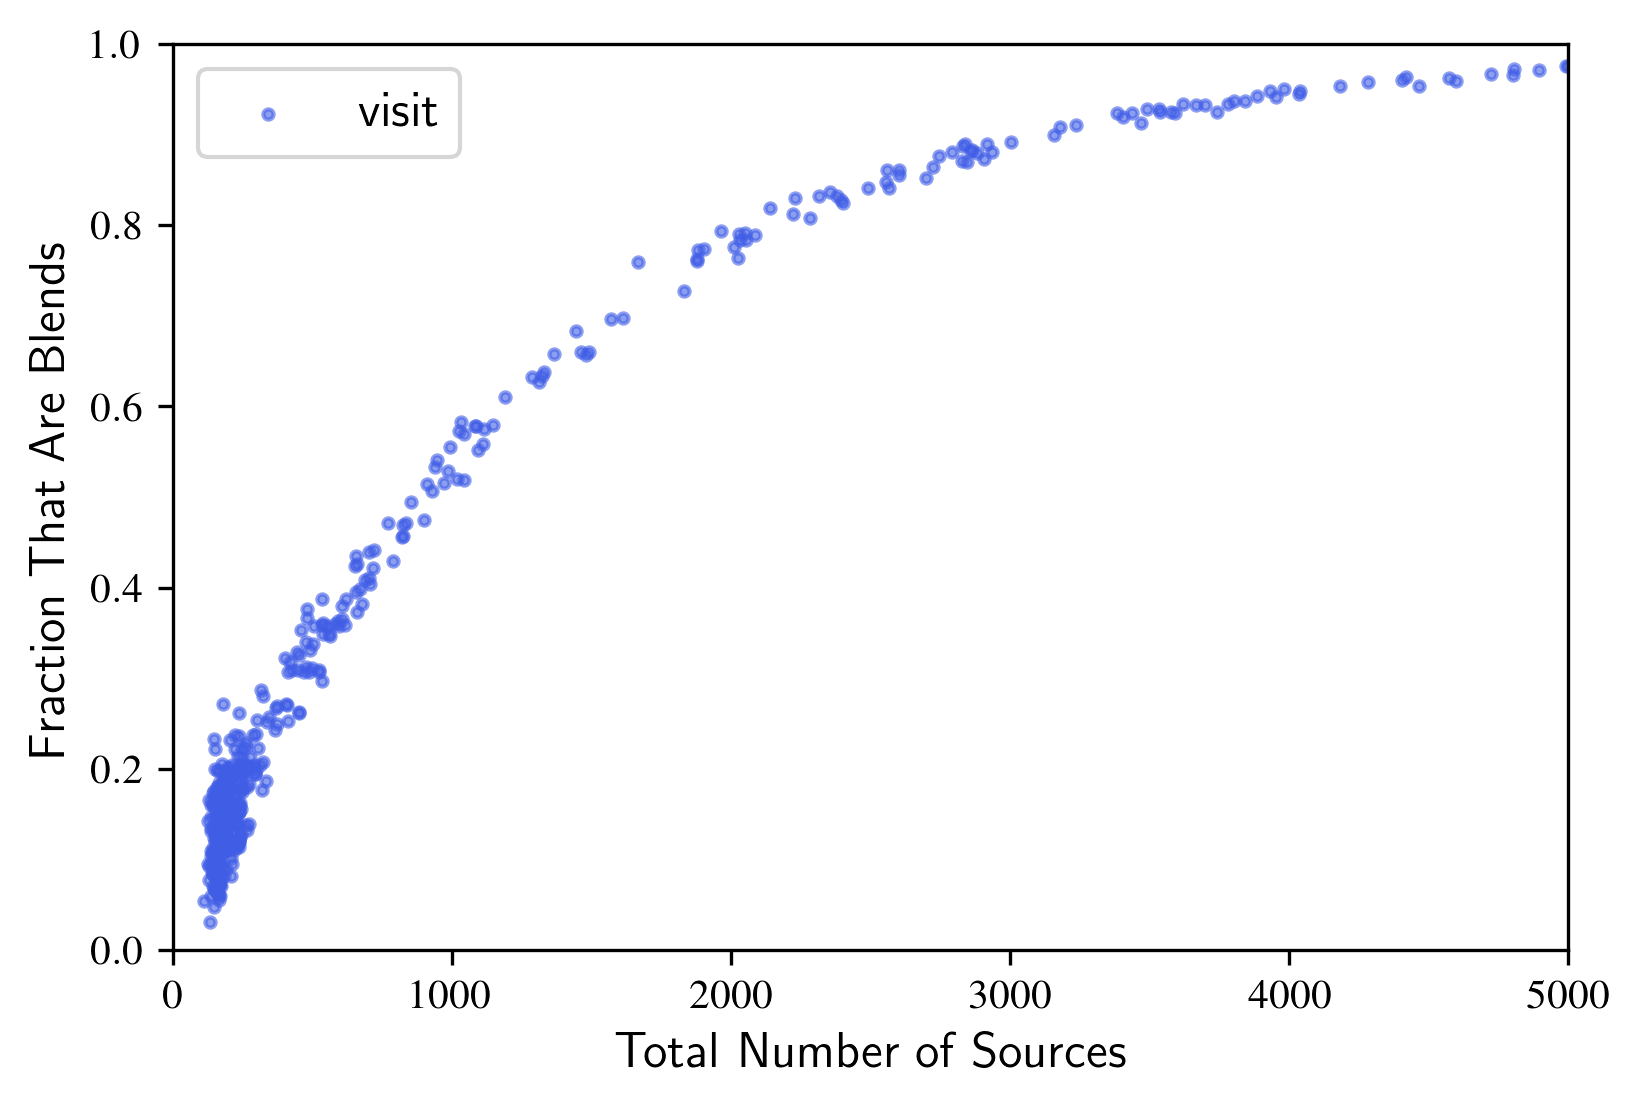
\includegraphics[width=\textwidth]{figs/simulating_donuts/blendfraction.png}
\end{tabular}
\end{center}
\caption[Fraction of Blended Sources]{The fraction of sources that are blends versus the total number of sources for the 497 visits in the full visit dataset.\label{fig:blendfraction}}
\end{figure}

% Full title as you would like it to appear on the page
\chapter{Training a Convolutional Neural Network To Predict The Local Wavefront}
\label{chap:cnn}
\chaptermark{Training a CNN}

\epigraph{Uncrumpling paper balls is what machine learning is about: finding neat representations for complex, highly folded data manifolds.}{Fran\c{c}ois Chollet}

In the first step, we use a convolutional neural network (CNN) to predict the relationship between donuts and their corresponding local wavefronts. There are three inputs to the network: the $256\ \times\ 256$ pixel donut image $D$, the position $r$ of the sensor. This position $r = (x,y,d)$ is comprised of the $(x,y)$ field position in radians, and the offset $d$ along the z-axis indicating whether the defocus is intra-focal or extra-focal. The output is the vector of Zernike coefficients $\alpha \in \mathbb{R}^{18}$. The sub-problem is to find a function approximator $\phi$,

\begin{equation*}
\phi(D, r) \to \alpha(x,y) \text{ such that } W(u,v|x,y) \approx \sum_{j=4}^{21}\alpha_j(x,y)Z_j(u,v)
\end{equation*}

Predicting the local wavefront $W(u,v|x,y)$ from donuts and their metadata is an intrinsically challenging problem because the optics contribution to the image is sometimes degenerate with, and typically subdominant to, the atmospheric contribution. Thus, even for very bright donuts with no effective sources of background noise, the model will have a systematic ceiling. In this section, we demonstrate that a CNN can produce accurate estimates despite this challenge.

\section{Network Architecture}

\begin{figure}[!htbp]
\begin{center}
\begin{tabular}{c}
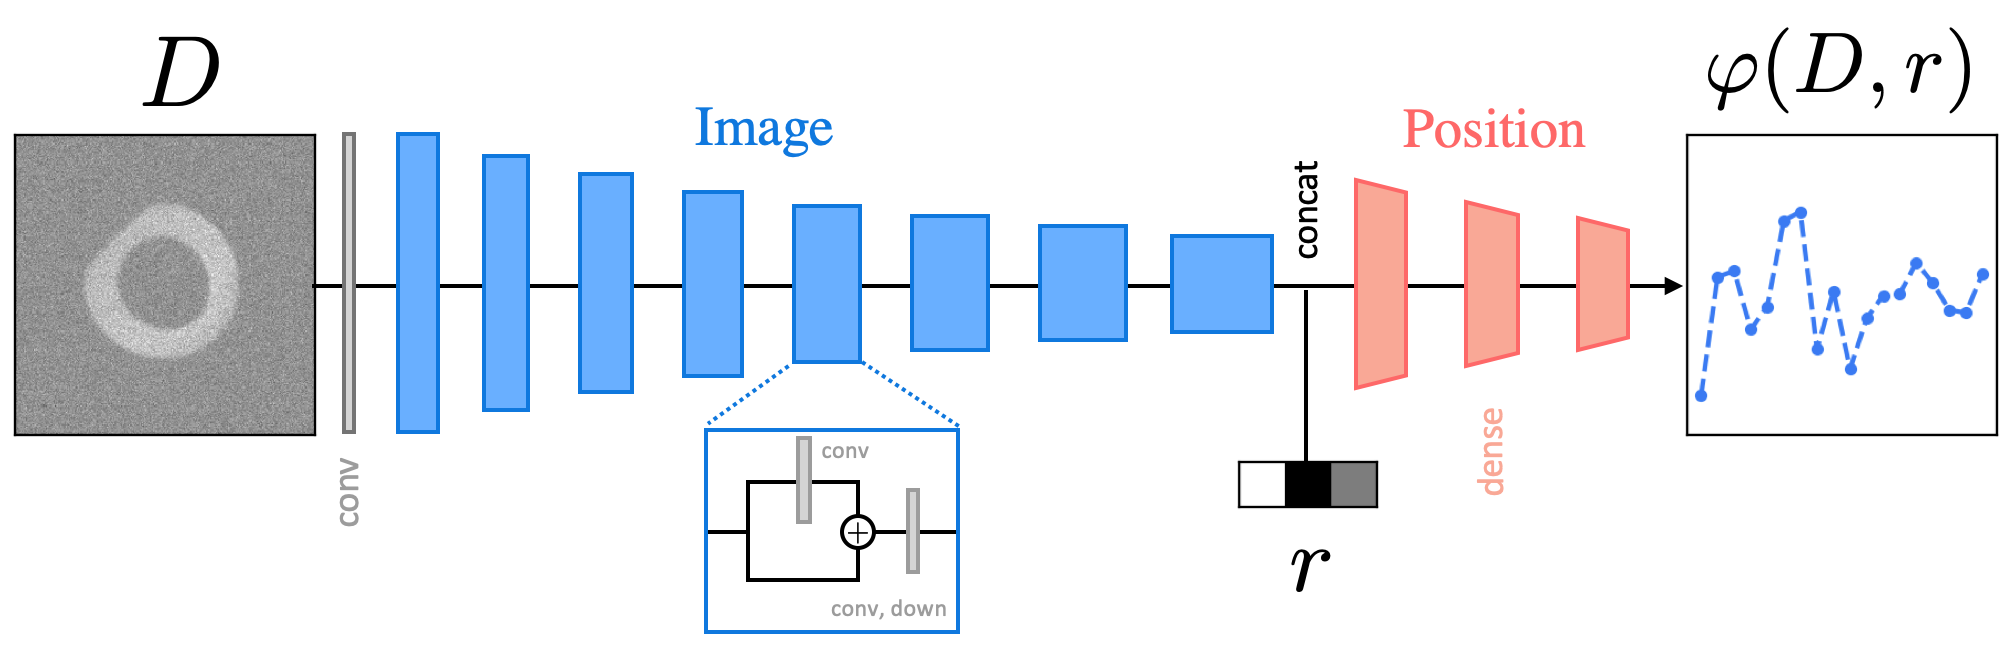
\includegraphics[width=\textwidth]{figs/cnn/arch.png}
\end{tabular}
\end{center}
\caption[Network Architecture]{The network architecture and example inputs and output. The image network is in blue and the position network is in red.\label{fig:arch}}
\end{figure}


Modern CNN architectures are governed by an astounding number of design decisions and hyper-parameter options. Here we show that a simple network can make highly accurate wavefront estimates without many additional design or hyper-parameter optimizations. This shows that this step can also serve as a network in other optics algorithms.

The network, shown in Figure \ref{fig:arch}, has two sub-networks: an image network and a position network. e will describe the architecture through the convolutions that are applied and how they change the data tensors. Each 2-dimensional convolution or linear layer, except the final linear layer, is followed by a 2-dimensional batch normalization layer (batchnorm) and a rectified linear activation (ReLU) \cite{726791, batchnorm, relu}. The batch normalization protects against covariate-shift and provides weak regularization and the ReLU activation introduces non-linearity. 

The image network reduces the donut image to a 1024 dimensional vector. The first component is a convolution that increases the depth of the input from 1 to 8, and retains the 256 by 256 height and width. This is followed by a sequence of 8 Down-Blocks. Each Down-Block has an initial convolution that does not change the tensor dimensions, followed by a convolution that increases the depth by a factor of 2 and reduces the height and width by a factor of 2. There is a skip connection between these two convolutions for better gradient flow \cite{resnet}. In the 8th and final Down-Block, the depth is not increased. Thus by the end of these steps we have a depth of $\text{depth} = 8 \cdot 2^7 = 1024$ and $\text{height} = \text{width} = 256 \cdot 2^{-8} = 1$. This $1 \times 1 \times 1024$ output is a learned representation of the input image. In total, the image network has 28,326,360 trainable parameters.

The position network combines the $1 \times 1 \times 1024$ output from the image network vector with the 3-dimensional position input $r=(x,y,d)$ and estimates the 18 local wavefront coefficients. It first concatenates and flattens these tensors into a combined 1027-dimensional tensor. Then three linear layers reduce the dimensionality to 266, 69, and 18 respectively (the sequential dimensions are log-linear). After the first linear layer we insert a dropout layer with a 90\% keep probability \cite{10.5555/2999134.2999257} to improve generalization. In total, the position network has 293,801 trainable parameters. 

We developed the model in PyTorch \cite{pytorch}. We determined this balance of parameters between sub-networks through testing. In the next Section we describe how the network is trained. 

\section{Training, Validation, and Testing}

\begin{figure}[!htbp]
\begin{center}
\begin{tabular}{c}
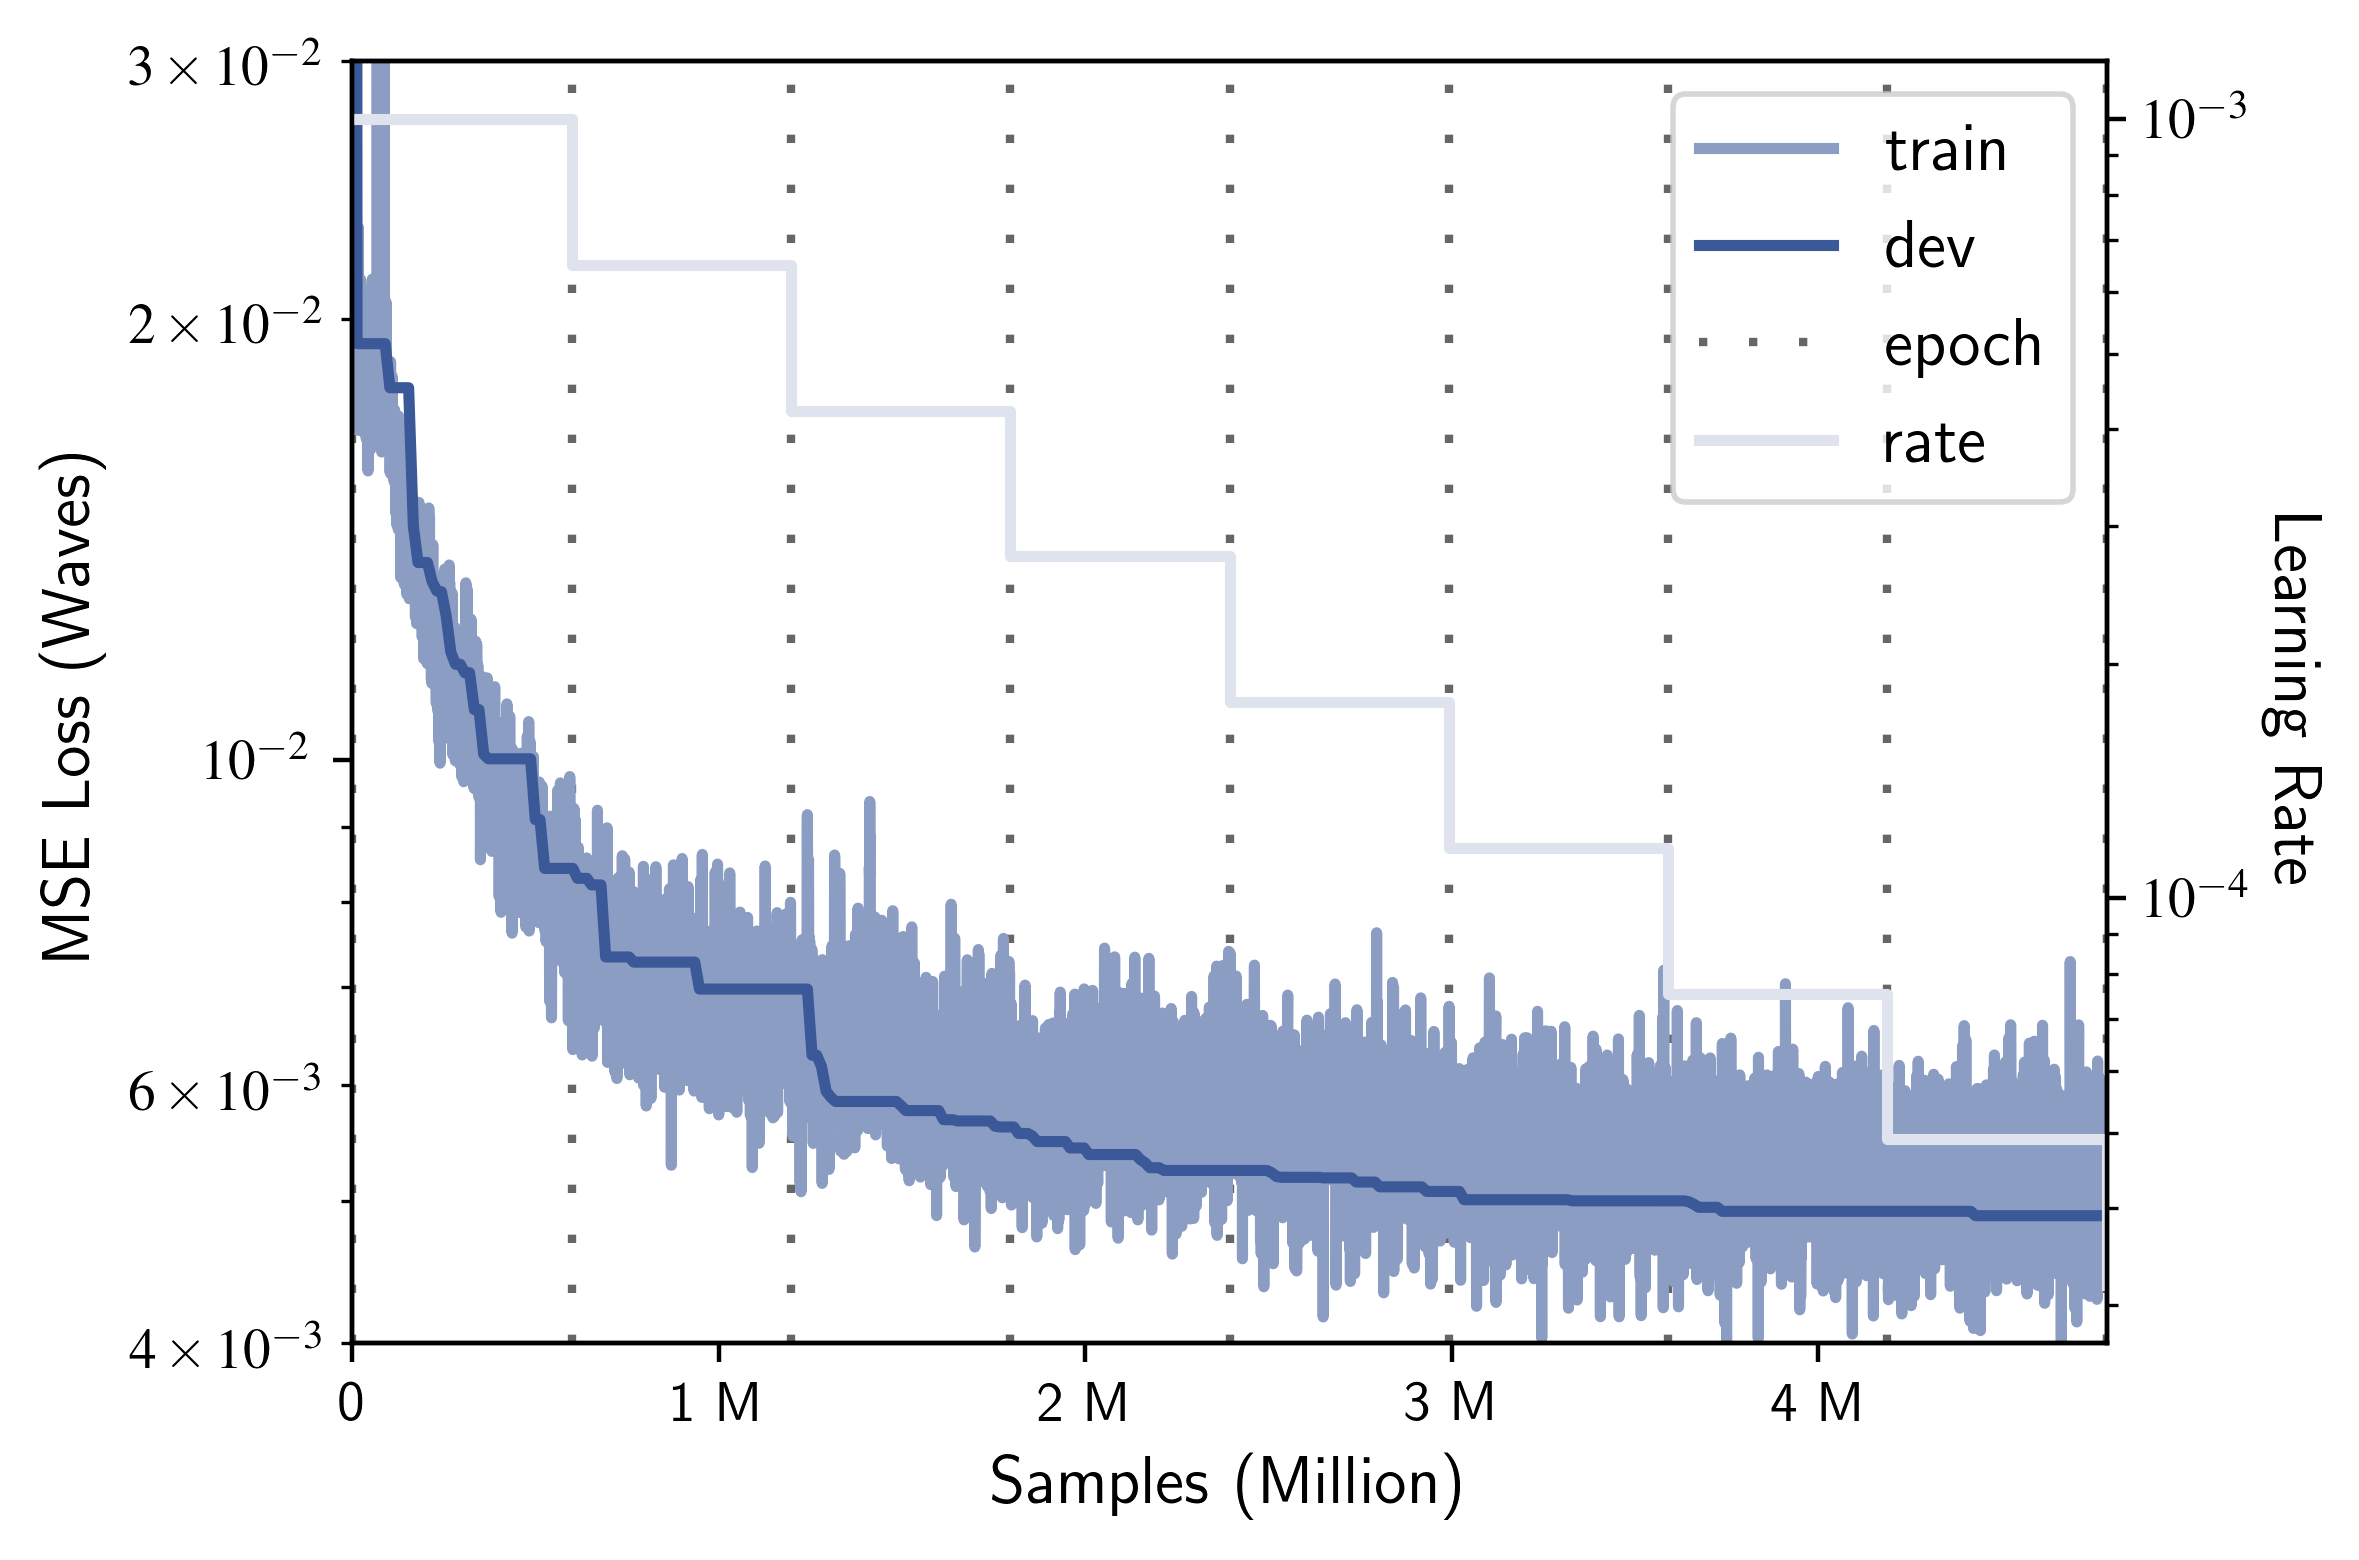
\includegraphics[width=\textwidth]{figs/cnn/training_curve.png}
\end{tabular}
\end{center}
\caption[Training Curve]{The training loss (train), validation loss (dev), and learning rate versus the number of samples used for training the neural network. The MSE loss corresponds to the y-axis on the left; the learning rate corresponds to the y-axis on the right.\label{fig:train}}
\end{figure}

In addition to the large number of decisions that go into the network architecture, there are also a lot of decisions on the configuration of the training. For the loss function, we use the mean-squared-error (MSE) between the estimated and true wavefront coefficients and found it to be superior to the mean-absolute-error. We evaluate batches of 64 samples at a time and use the Adam optimizer to compute the parameter updates for the backward pass after computing the loss function in the forward pass \cite{adam}. We train the model for 8 epochs over the donut dataset. After each epoch we multiply the learning rate by a factor of 0.65. Every 200 batches, we evaluate the MSE of the model on the donut validation set, and keep the best model. Figure \ref{fig:train} shows the training and validation (dev) errors, and the learning rate, versus the number of training samples.

\begin{figure}[!htbp]
\begin{center}
\begin{tabular}{c}
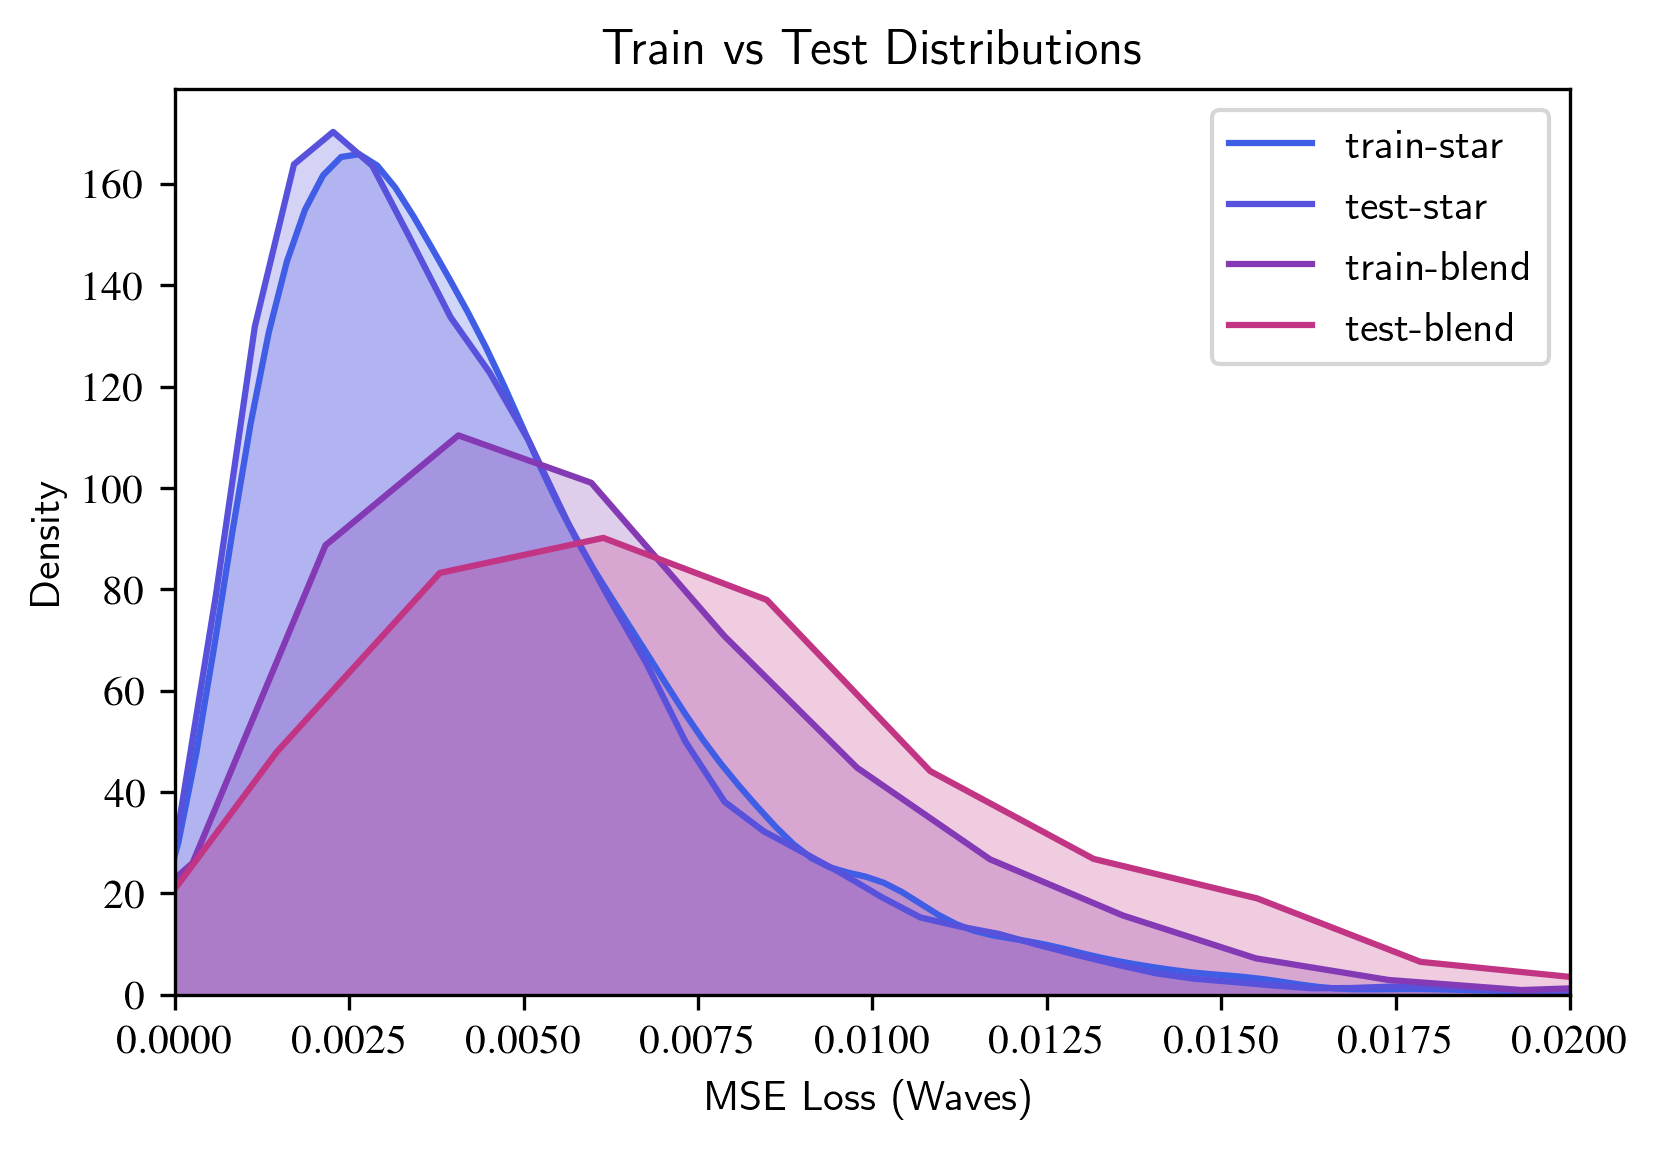
\includegraphics[width=\textwidth]{figs/cnn/train_vs_test.png}
\end{tabular}
\end{center}
\caption[Train Versus Test MSE Loss]{The distributions of the training and test MSE loss on stars (donuts with no overlaps) and blends (donuts with overlaps).\label{fig:train_vs_test}}
\end{figure}

We went through multiple iterations with different training configurations to arrive at this final configuration. To assess the models we used the validation set. Once we finalized the training configuration, we used the held out test set for a final assessment of the network. We compared the MSE loss on the training and test sets to check for overfitting. Figure \ref{fig:train_vs_test} shows the comparison. The training and test set MSE losses are $4.5\pm 3.2$ and $4.4\pm 3.5$ thousandths of waves on stars respectively, and $9.5\pm 20.0$ and $9.6\pm 22.0$ thousandths of waves on blends respectively. The performance on the training and test sets is almost identical, which suggests our model is not overfitting.

\begin{figure}[!htbp]
\begin{center}
\begin{tabular}{c}
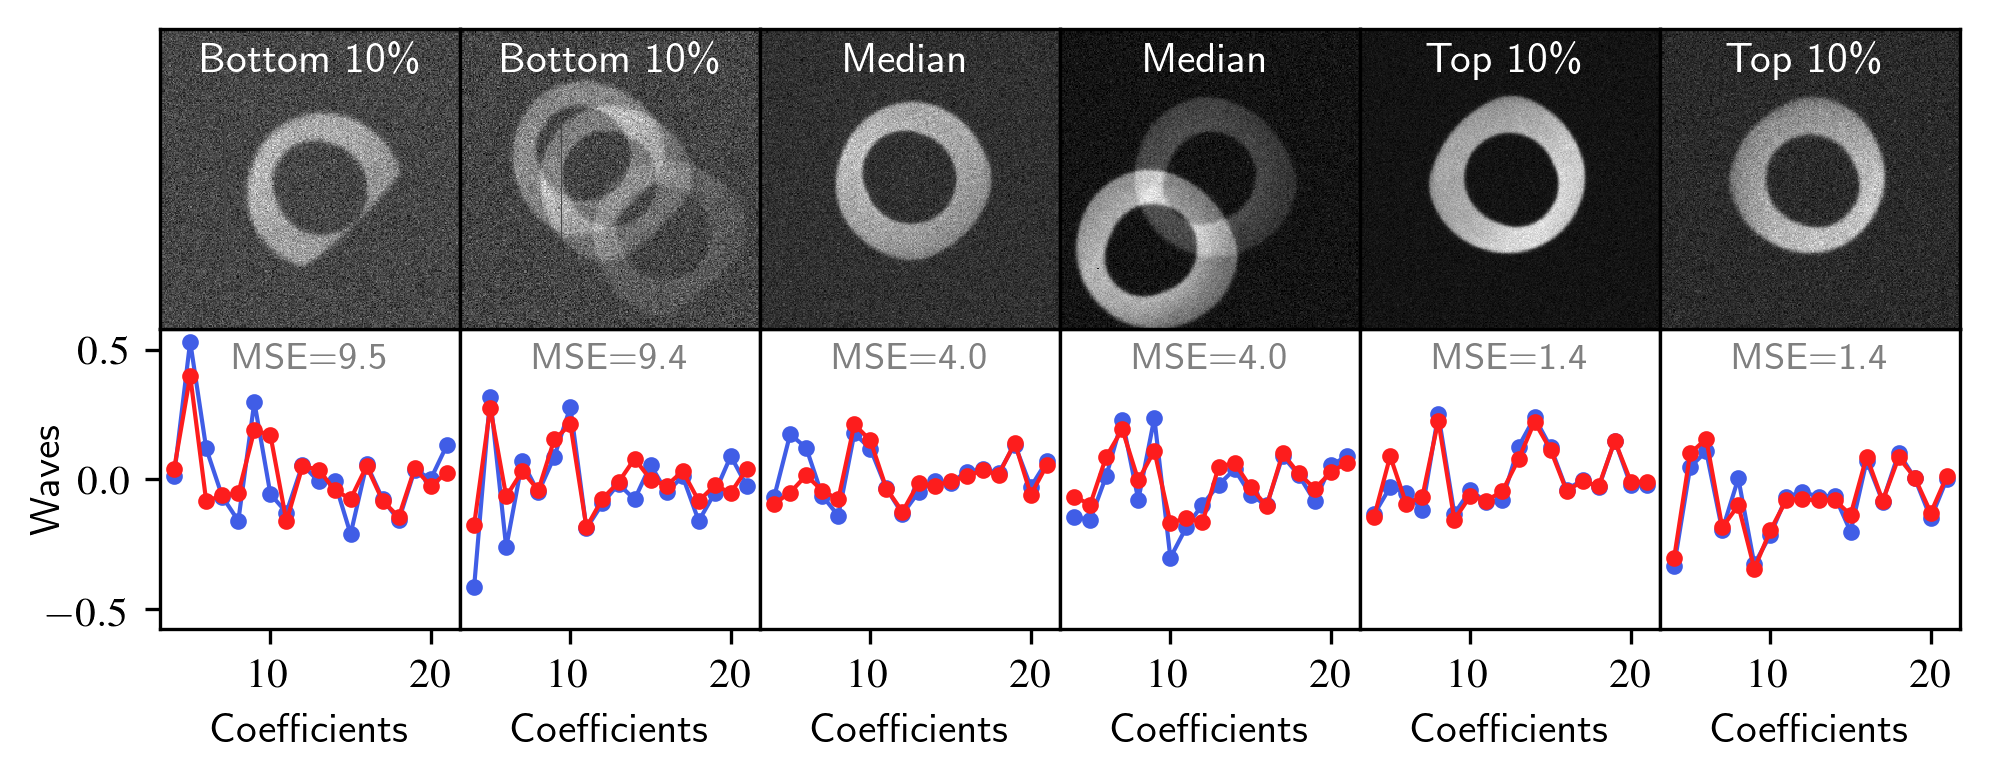
\includegraphics[width=\textwidth]{figs/cnn/donut_panel_test.png}
\end{tabular}
\end{center}
\caption[Panel of Donut Results]{Top: six donut images; two from the bottom 10\% of the MSE distribution, two from the median, and two from the top 10\%. Bottom: the corresponding true (blue) and neural network estimated (red) local wavefronts. The MSEs in the bottom row are in units of thousandths of waves.\label{fig:donut_panel}}
\end{figure}

We also inspected the performance of the network on many samples. Figure \ref{fig:donut_panel} shows the performance on six donuts from across the MSE loss distribution. At the bottom decile, the network achieves a MSE of 9.5 thousandths of a wave. While benchmarks do not exist for this task, based on our experience with other approaches and previous generation telescopes, this already seems like a competitive result. The median MSE is 4.0 thousandths of a wave. Here a few differences between the true and estimated coefficients can be seen by eye. At the top decile, the network achieves a MSE of 1.4 thousandths of a wave. The match between the true and estimated coefficients is astounding. It is perhaps more astounding to consider that the network is able to achieve this when the optics contribution that we are estimating is sub-dominant to the atmospheric contribution. 

\begin{figure}[!htbp]
\begin{center}
\begin{tabular}{c}
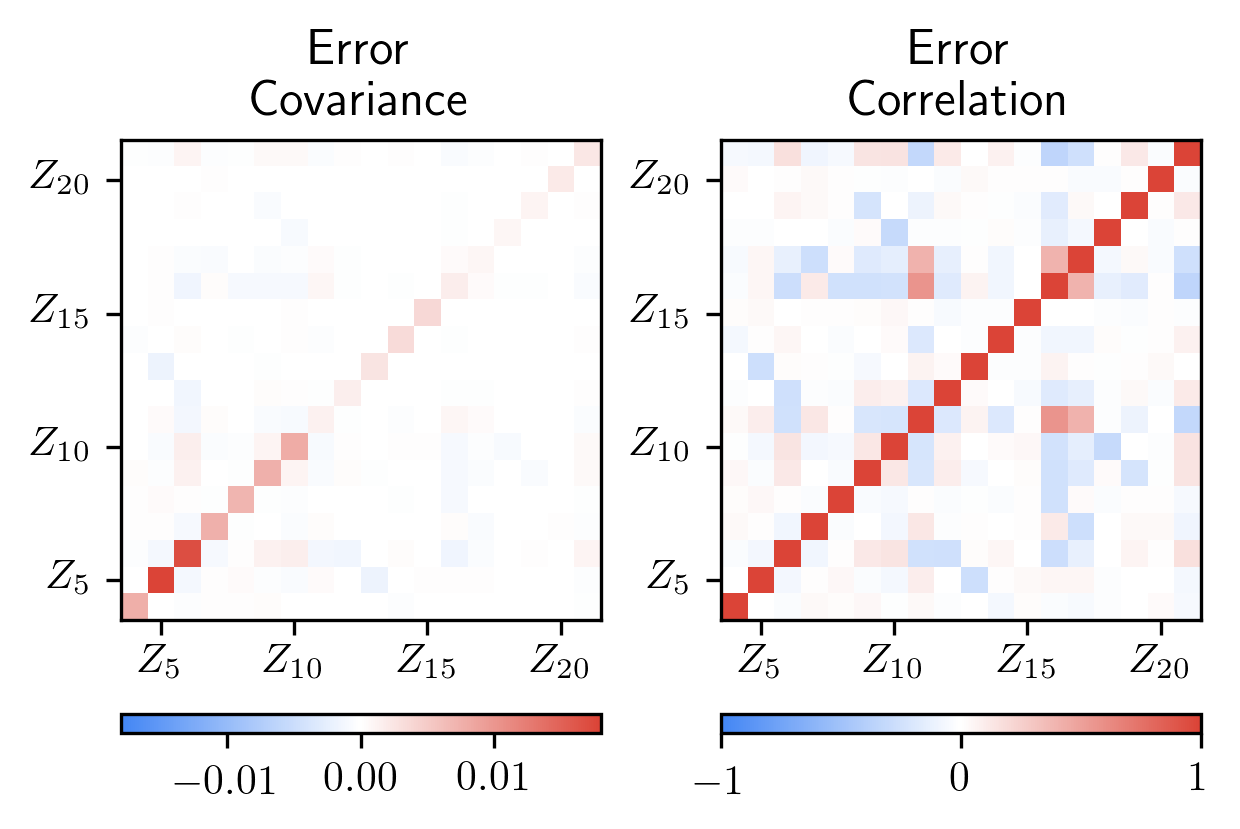
\includegraphics[width=\textwidth]{figs/cnn/cov_cor.png}
\end{tabular}
\end{center}
\caption[Wavefront Coefficient Error Covariance and Correlation]{The covariance (left) and correlation (right) of the error between different local wavefront coefficients.\label{fig:cov_cor}}
\end{figure}

It is also important to examine the correlation between the errors on different wavefront coefficients to see if there are systematic errors and biases. Figure \ref{fig:cov_cor} shows the covariance and correlation matrices for the error on the different wavefront coefficients. The covariance diagonal matches with the coefficients that are most excited in our donut dataset. For example, the $Z_5, Z_6$ astigmatism coefficients have the largest error, but also have the largest values in the true wavefront. The correlation matrix shows that the errors are fairly independent across coefficients. The largest correlations are 0.57 between $Z_{11}, Z_{16}$; 0.41 between $Z_{11},Z_{17}$; 0.40 between $Z_{16},Z_{17}$; and -0.34 between $Z_{16}, Z_{21}$.

There are a lot of parameters that determine a donut image. Another natural question is whether any of these are correlated with the error. Figure \ref{fig:err_sources} shows 8, out of the many, error sources we examined. We found that the error generally increases when the background noise increases or foreground number of photons in the donut decreases, as expected. The ratio of these contributions serves as a proxy for the signal-to-noise ratio.

Interestingly, the seeing does not have much impact, suggesting that the network is really able to differentiate between PSF contributions due to the atmosphere and due to the optics. Before training the network, we had also expected the radial distance, a proxy for the amount of vignetting, to be correlated with the error. However, in practice, it seems like the network is able to utilize the $(x,y)$ coordinates in the position to account for this effect and process vignetted donuts accurately.

\begin{figure}[!htbp]
\begin{center}
\begin{tabular}{c}
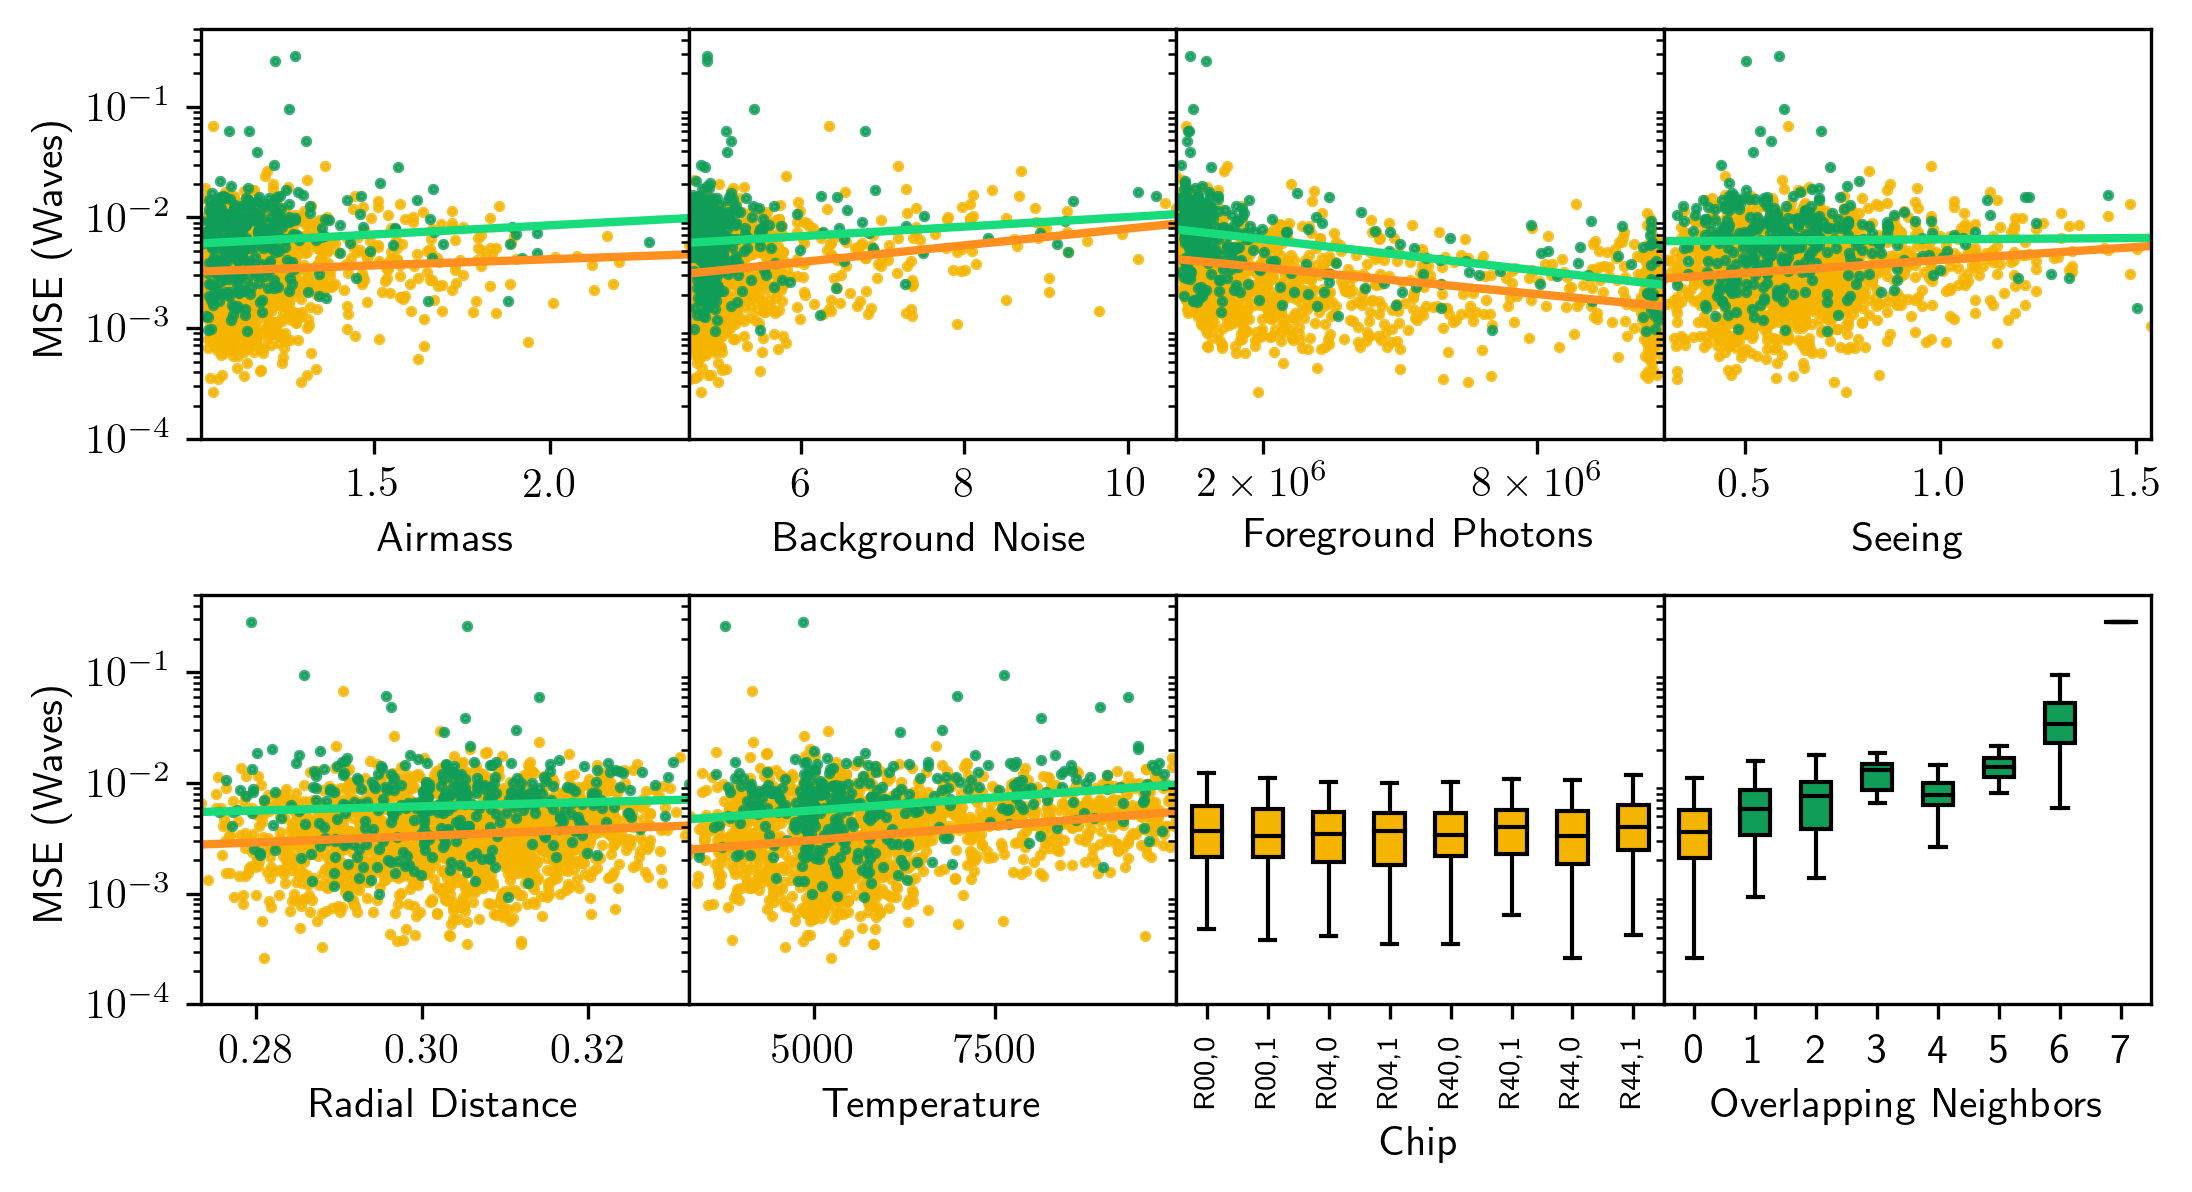
\includegraphics[width=\textwidth]{figs/cnn/error_analysis.png}
\end{tabular}
\end{center}
\caption[Panel of Potential Sources of Error]{The MSE, in waves, versus the feature distributions for 8 different potential sources of error. The stars are highlighted in yellow; the blends are in green. We also show the best fit line for the 6 non-categorical features. Units: Background Noise is the standard deviation of photons in the background, Foreground Photons is the total number of photons in the donut, Seeing is in arcseconds, Radial Distance is in meters, Temperature is in Kelvin. \label{fig:err_sources}}
\end{figure}

The biggest surprise was the impact of chromatic effects. The temperature of the source is reasonably correlated with the error. The fact that there is also some error correlation with airmass suggests some of this stems from differential chromatic refraction and some from the variations in wavelength across Rubin's r-passband and how this contributes to PSF structure. In future versions of this model, one could imagine training the network to also predict the temperature, or peak wavelength, of the source. This would better encourage it to differentiate the chromatic effects during training.

Finally, there is a clear difference between the stars (sources with no overlaps) and blends (sources with overlaps). The network performs much worse on the blends. This has important implications for which sources, and even fields, to do wavefront sensing in. As the number of overlapping neighbors increases, the error increases. However, it is important to note that there are fewer samples with large numbers of overlapping neighbors so these distributions are less reliable. In Section \ref{chap:interp}, we explore whether ignoring blends improves the performance of the global wavefront interpolation.

\section{Neural Network Enabled Insights}

At a high level, neural networks are differentiable and parameterized function approximators. The same properties that make them trainable, make them effective tools for exploring tasks in new ways. Here our network $\varphi$ has been trained to solve the task $\varphi(D, r) = \alpha$. In the next three subsections, we perform mathematical manipulations on $\varphi$ to gain insight into the behavior of our network and more general properties of this problem.

\subsection{Saliency Maps}

What aspects of the donut images is the neural network using to make its predictions? Following in the footsteps of \cite{saliency}, we define a metric that shows the pixels the predictions of the network are most sensitive to. We call this \textit{attention} and compute it by taking the magnitude of the gradient of the norm of the local wavefront prediction with respect to \textit{the pixels}. The explicit formula is

\begin{equation*}
\text{Attention}\ = \left|\nabla_D || \varphi(D, r)||_2 \right|
\end{equation*}

\noindent This gradient with respect to pixels is similar to the mechanism behind style transfer \cite{style_transfer}. 

\begin{figure}[!htbp]
\begin{center}
\begin{tabular}{c}
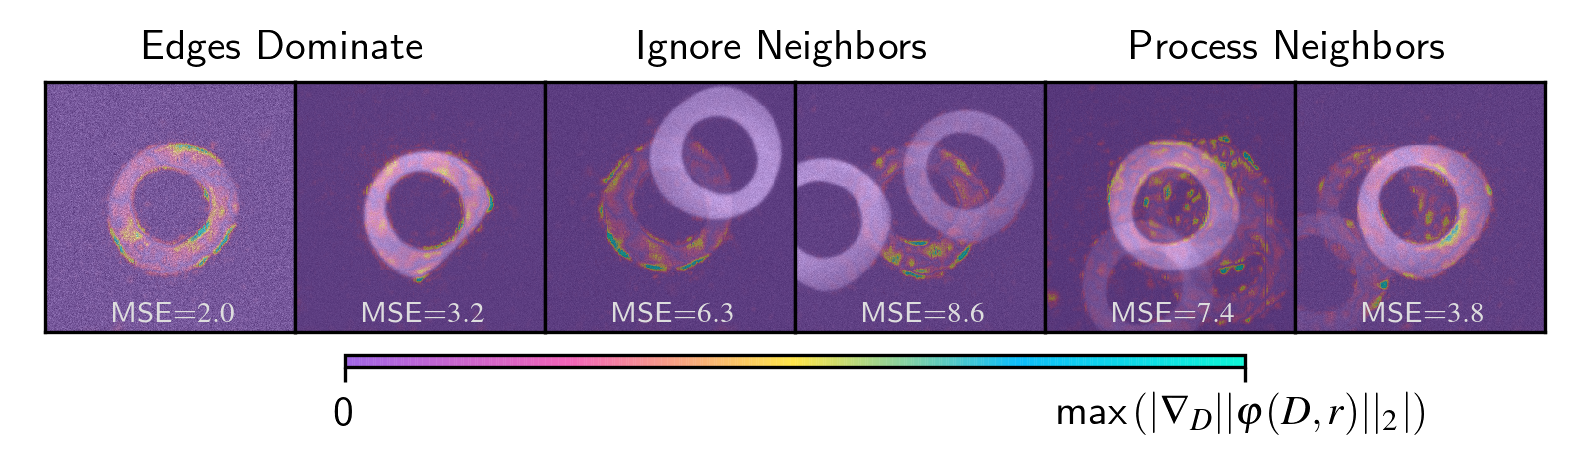
\includegraphics[width=\textwidth]{figs/cnn/attention.png}
\end{tabular}
\end{center}
\caption[Neural Network Attention]{The neural network attention values for six samples.\label{fig:attention}}
\end{figure}

Figure \ref{fig:attention} shows the attention for six samples. The first pattern that emerges is that the edges dominate, particularly when there is significant vignetting. The network focuses on the outline of a donut, in tandem with its position, to determine the wavefront. This suggests it may be possible to develop a successful network that takes only the outline of the donuts as input. It is not clear how we would have picked up this insight from the other approaches. This is an example of how the neural network can teach us new things about a problem and help us discover new approaches. 

The second pattern is that, in the case of blends, the network either utilizes or ignore the neighboring donuts. It is curious that this behavior is so bimodal. For example, where in the network is this decision being made? We suspect answering this question could unlock ways to further improve the performance of the network on blends. 

\subsection{Memorizing Versus Learning}

A common grievance of opponents to machine learning being applied in physics is that the network is memorizing, rather than truly learning, the relationships between the input and output. Here, we test this. We examine the intensity changes that would most quickly move the predictions on a base donut towards the Zernike of interest, which we deem the label-shift. We take the gradient of the norm of the difference of the network output and the target Zernike unit vector, or explicitly

\begin{equation*}
\text{Label-Shift}\ = \nabla_D || \varphi(D, r) - Z_i||_2
\end{equation*}

Figure \ref{fig:label-shift} shows the results for the Zernike unit vectors $Z_4$ through $Z_{21}$ under the respective annular Zernike polynomial. The similarity between the intensity changes and the Zernike polynomials is striking, especially given that the network has not been explicitly trained to learn these patterns. For example, the network even learns the 5 cycle periodicity of $Z_{20}$ and $Z_{21}$. It also learns the complicated radial dependence of $Z_{18}$. This demonstrates that the network is engaging in higher order learning, where it is learning general features of the problem space.

\begin{figure}[!htbp]
\begin{center}
\begin{tabular}{c}
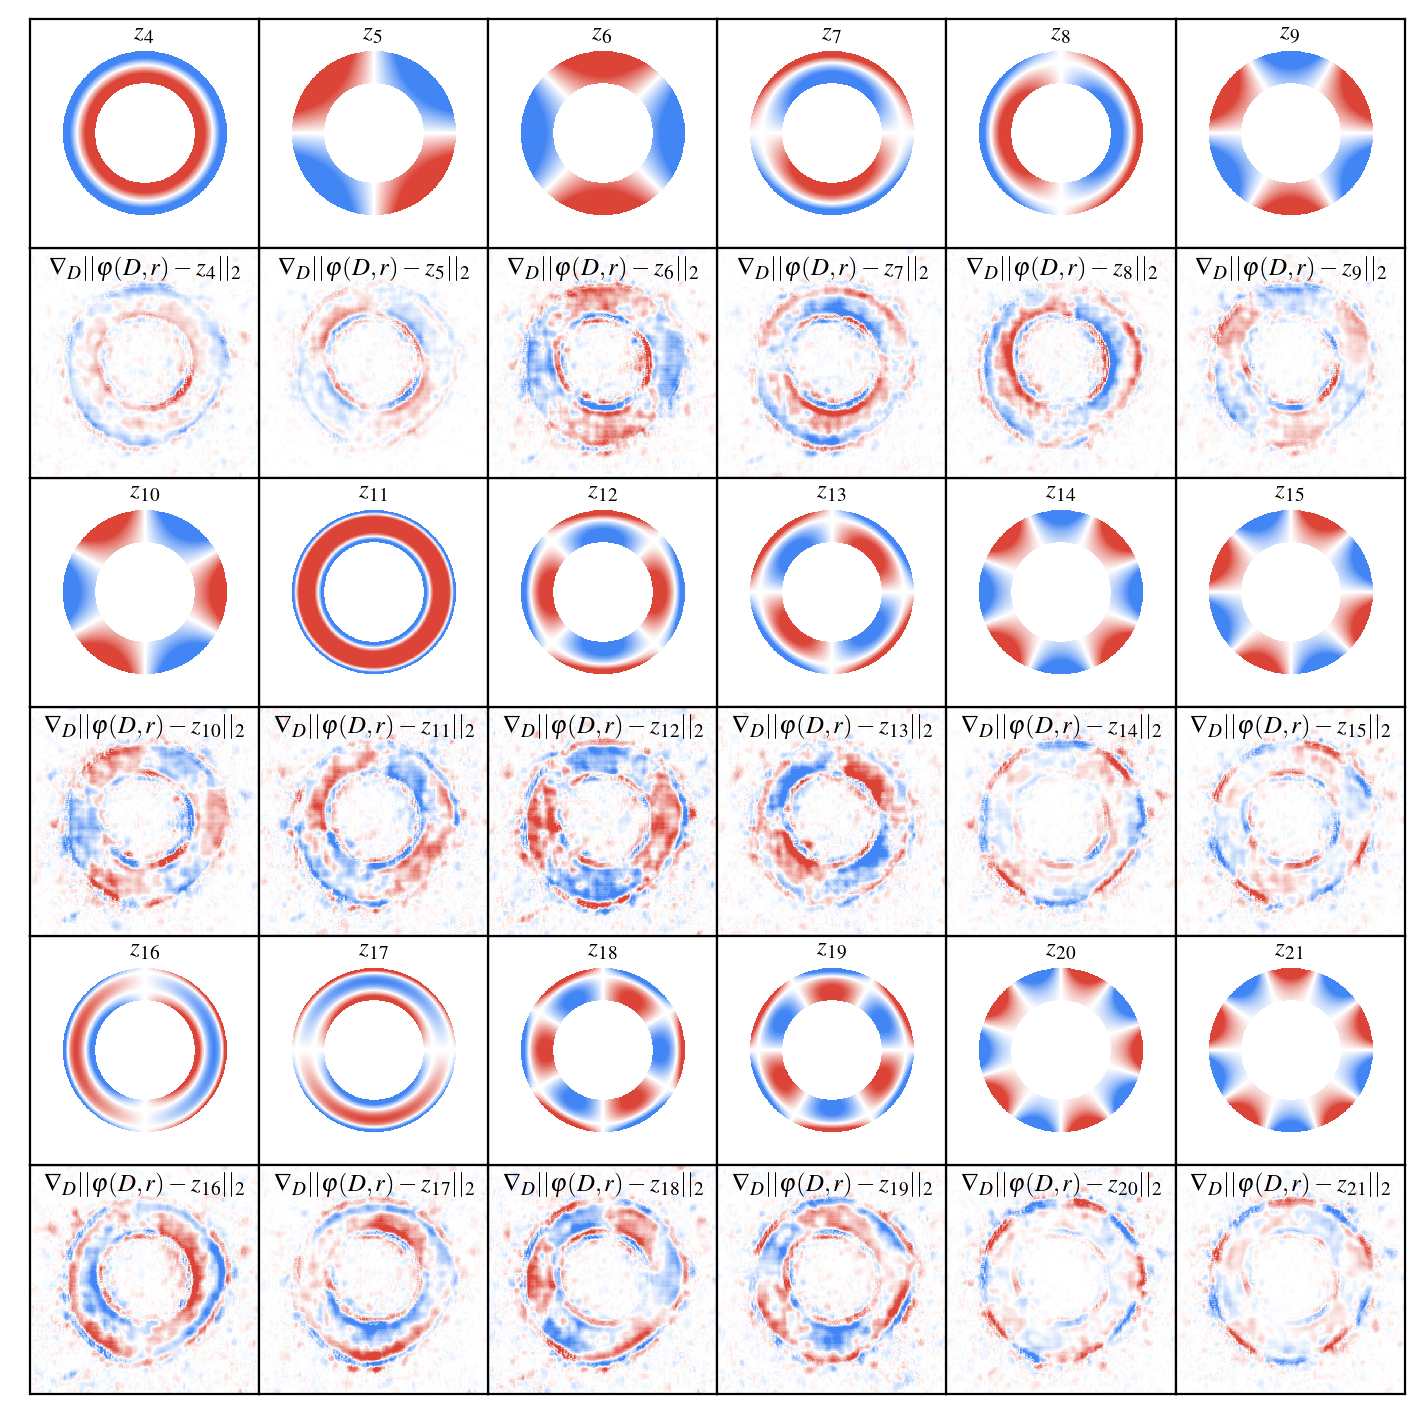
\includegraphics[width=\textwidth]{figs/cnn/morph.png}
\end{tabular}
\end{center}
\caption[Neural Network Label-Shifts]{The odd rows show the annular Zernike polynomials $Z_4$ through $Z_{21}$. The even rows show the neural network label-shifts for the corresponding Zernike unit vectors. \label{fig:label-shift}}
\end{figure}

\subsection{Adversarial Tradeoffs}

The input space for our problem, the image and the position, has $256 \times 256 + 3 = 65539$ dimensions. This is an extremely high dimensional space. It is not hard to find subtle changes in this space that are hardly discernable \textit{by eye}, or at a global level, but which can dramatically change the output of the network. In \cite{2014arXiv1412.6572G}, the authors show how to use these adversarial examples to improve training. Here, we examine a few adversarial examples to understand how our network could be hacked. 

An attacker has two competing objectives. The first is to find a modified donut image $D^\prime$ that is similar to $D$; the second is to find a modified donut image $D^\prime$ such that $\varphi(D^\prime, r)$ is close to some target $t^\prime \in \mathbb{R}^{18}$. The Adversarial-Objective is,

\begin{equation*}
\text{Adversarial-Objective}\ = ||\varphi(D^\prime, r) - t^\prime||_2^2 + ||D - D^\prime||_2^2
\end{equation*}

\noindent In order to find such a $D^\prime$ we can minimize this objective function with respect to $D^\prime$. We use the Adam optimizer to perform gradient descent. Two example results are shown in Figure \ref{fig:adversarial}. In both cases we only change one coefficient in the target $t^\prime$. 

\begin{figure}[!htbp]
\begin{center}
\begin{tabular}{c}
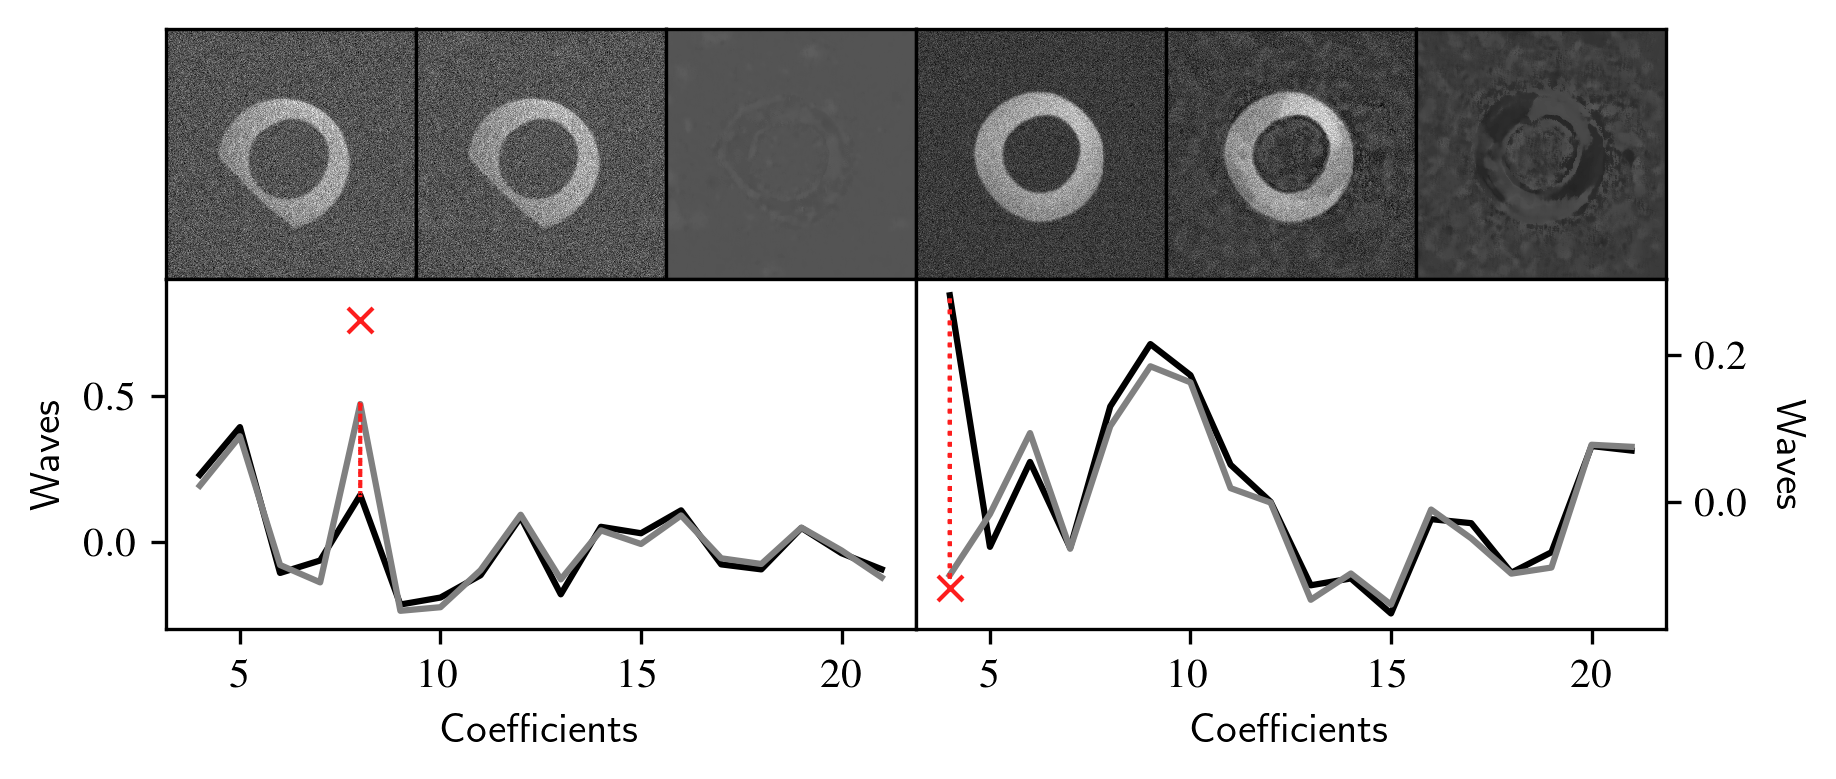
\includegraphics[width=\textwidth]{figs/cnn/adversarial.png}
\end{tabular}
\end{center}
\caption[Adversarial Attack]{Two example adversarial attacks. For each of the attacks we show three donut images, from left to right: the original donut image $D$, the new donut image $D^\prime$, and the difference $D^\prime - D$. Below we show the original prediction $\varphi(D,r)$ in black, the target $t^\prime$ as a red ``x'', and the new prediction $\varphi(D^\prime, r)$ in gray.\label{fig:adversarial}}
\end{figure}

In practice, one must scale the ratio of the two terms in the Adversarial-Objective to get good convergence. This ratio determines the relative priority of similarity between $D$ and $D^\prime$ versus $\varphi(D^\prime, r)$ and $t^\prime$. In the example on the left, we prioritized the similarity of the donuts. Here, the two donuts appear the same by eye. However, the coefficient for $Z_8$ is increased significantly, although not all the way to the target - while keeping most of the other coefficients close to their original values. This highlights the power of this kind of attack.

In the second example, the difference between the donut images is clearly discernible. Here the $Z_4$ coefficient changes dramatically, and largely hits the target, and even changes signs. This shows how the prediction can be manipulated to the target with sufficient changes to the donut. 

In the context of the Rubin Observatory, a closed environment, adverse attacks need not be feared. However, the algorithm we develop here serves a general building block for other wavefront sensing methods. These algorithms are also used for defense purposes. In this context, the sensitivity to adversarial attacks is an important characteristic to be aware of, and potentially protect against.


% Full title as you would like it to appear on the page
\chapter{Long paper 1 chapter title}
\label{chap:interp}
\chaptermark{Foo}

\epigraph{It doesn't matter how beautiful your theory is, it doesn't matter how smart you are. If it doesn't agree with experiment, it's wrong.}{Richard P. Feynman}
% \epigraph{The first principle is that you must not fool yourself and you are the easiest person to fool.}{Richard P. Feynman}


\section{Abstract}
Concise introduction, motivation, results, and conclusions.

\section{Introduction}
Examples of citations: we knew X from \cite{Croote201616022} and Y from \cite{Croote20181306}.

\section{Results}
\subsection{Result 1}
Here is a reference to Figure \ref{fig:paper1_fig1}.
We found bacteria, roughly 5 \si{\mu}m in length, that live at 95\degree C for roughly 90\% of the year. More symbols: \$, \#, 10\textsuperscript{5}, $\alpha$, $\beta$, $\gamma$, $\kappa$, \textbf{bold}, \textit{italics}.
Quotation marks are "correctly oriented" thanks to the csquotes package.
Now an inline equation: $E = mc^2$. Now a reference to Equation \ref{eqn:paper1_eqn1}:
\begin{equation}\label{eqn:paper1_eqn1}
d_t = \frac{c - pn_t}{n_t}
\end{equation}

\begin{figure}[hbt!]
\centering
\includegraphics[width=14cm, keepaspectratio]{figs/paper1/fig1.png}
\caption[Short figure caption for List of Figures]{Long figure caption text that explains everything.}
\label{fig:paper1_fig1}
\end{figure}

There will be more text here.

More text here.

More text here.

More text here.

More text here.

More text here.

\subsection{Result 2}
We discovered something else. Here is a reference to Table \ref{tab:paper1_tab1}.

\renewcommand{\arraystretch}{2}  % make spacing nicer
\begin{table}[hbt!]
\centering
\begin{tabularx}{\textwidth}{c|c|c|c}  % 4 columns center-justified
   \textbf{Col 1} & \textbf{Col 2} & \textbf{Col 3} & \textbf{Col 4} \\
   \hline  % horizontal line
   Text in Row 1a & Text in Row 1b & Text in Row 1c & Lots of text in Row 1d \\
                  & Row 1.5b & Row 1.5c & Row 1.5d \\
   \hline
   Row 2a & Row 2b & Row 2c & Row 2d \\
   \hline
   Row 3a & Row 3b & Row 3c & Row 3d \\
\end{tabularx}
\caption[Short table caption for List of Tables]{Long table caption explaining everything.}
\label{tab:paper1_tab1}
\end{table}

More text here.

More text here.

More text here.

More text here.

\begin{sloppypar}
FixAwkwardSpacingWithSloppypar FixAwkwardSpacingWithSloppypar FixAwkwardSpacingWithSloppypar FixAwkwardSpacingWithSloppypar FixAwkwardSpacingWithSloppypar.
\end{sloppypar}

More text here.

More text here.

\section{Conclusions}
The end of the paper.

% Full title as you would like it to appear on the page
\chapter{Long paper 1 chapter title}
\label{chap:err}
% Short title that appears in the header of pages within the chapter
\chaptermark{Short chapter title}

\section{Conclusions}
The end of the paper.

% Full title as you would like it to appear on the page
\chapter{Conclusion}
\label{chap:conclusion}
% Short title that appears in the header of pages within the chapter
\chaptermark{Short chapter title}

\section{Conclusions}
The end of the paper.

% \part{Star Trail Photometry}
% \part{Quantum Metric Learning}

% \include{ch_conclusion}

% uncomment below if you have an appendix
% \appendix
% \chapter{A Long Proof}

\bibliographystyle{unsrt}  % can change to fit your field e.g. pnas2009
\bibliography{mybib}  % no .bib extension necessary

% adds a non-numbered signature page at end (for printing on ACID-FREE paper)
% (remember to comment out when submitting final version)
\onlinesignature

\end{document}
